\documentclass[11pt]{article}

\usepackage[utf8]{inputenc}
\usepackage[T1]{fontenc}
\usepackage{lmodern}
\usepackage[margin=1in]{geometry}
\usepackage{amsmath,amssymb,amsthm}
\usepackage{booktabs}
\usepackage{tabularx}
\usepackage{longtable}
\usepackage{array}
\usepackage{enumitem}
\usepackage{microtype}
\usepackage[hidelinks]{hyperref}
\usepackage{xurl}
\usepackage{graphicx}

\newcolumntype{L}{>{\raggedright\arraybackslash}X}
\renewcommand{\arraystretch}{1.15}
\setlist{itemsep=2pt}
\setlength{\emergencystretch}{3em}

\DeclareMathOperator{\mean}{mean}
\newcommand{\E}{\mathbb{E}}
\newcommand{\eps}{\varepsilon}
\newcommand{\KL}{\mathrm{KL}}
\newcommand{\poly}{\mathrm{poly}}

\theoremstyle{plain}
\newtheorem{lemma}{Lemma}
\newtheorem*{theorem*}{Theorem}
\newtheorem{theorem}{Theorem}
\newtheorem{proposition}{Proposition}
\newtheorem{conjecture}{Conjecture}
\newtheorem*{proposition*}{Proposition}
\newtheorem*{conjecture*}{Conjecture}

\hypersetup{
  pdftitle={A certified exponent of 0.48758 for worst-case Subset Sum, and limits of the alias-checksum analysis},
  pdfauthor={Jennifer Voitle}
}

\begin{document}

\title{A certified exponent of 0.48758 for worst-case Subset Sum, and limits of the alias--checksum analysis}
\author{Jennifer Voitle\\ Independent researcher}
\date{Draft, 5 November 2026}

\maketitle

\begin{abstract}
For more than fifty years, since Horowitz and Sahni's meet-in-the-middle algorithm of 1974, the best exponent for worst-case Subset Sum was $1/2$. In October 2026 that barrier fell twice within a week, with OpenAI's $2^{0.49n}$ algorithm and, independently, Li and Ye's $2^{(1/2 - 1/450000)n} \approx 2^{0.4999978n}$, and improvements have followed quickly since: within three weeks A.~Kapila's modification of the OpenAI approach (``Base'') reached 0.4877, and a retuning of Base by JoshuaQFEX reached 0.487676. Here we push this line of work further and examine what limits it. Conditional on the cited non-numerical proofs, we give a certified parameter point with threshold $T=0.4875754036$: for every fixed $T'>T$, the uniform randomized algorithm uses $O(2^{T'n})$ word operations on inputs of polynomial bit length, with success probability at least $2/3$. In particular, it runs in time $O(2^{0.4875755n})$. A single asymmetric filter replaces Base's family of 43 filters. Independent interval computations certify all required numerical conditions, including both filtering moments and their quadrature errors.

We prove a lower bound on the first filtering moment, valid for all positive continuous densities, that excludes every parameter choice with $\tau\le0.484$ in the original OpenAI proof's sufficient budget. Three algebraic bounds explain the costs at our improved point. Separately, an enumeration phase that inserts at least $2^{(1-\eta-o(1))n}$ alias classes, spending a counted step on each, and uses checksum gap at most $\Delta$ needs exponent at least $(1-\Delta)/2$. This is a conditional operation-count bound; a global upper bound on achievable checksum capacity remains open. Finally, we isolate a small-layer statement that would yield threshold $0.4873407528$, prove combinatorial special cases, and identify the remaining questions.
\end{abstract}

%======================================================================
\section{Introduction}

For more than fifty years, from Horowitz and Sahni's meet-in-the-middle algorithm in 1974~\cite{hs} until October 2026, the best exponent for worst-case Subset Sum was $1/2$. Then, within a few weeks, OpenAI and, independently, Li and Ye broke that barrier, and several further improvements appeared; the area is moving quickly. This paper asks how far one of the two new approaches, OpenAI's, can be pushed: we improve the best exponent in that line of work (Theorem~\ref{thm:main} below), explain what limits it near 0.4876, and state the open problems that would move it further. Two of our results concern the analysis as a whole rather than one parameter point (the terms are explained below). A lower bound on the first filtering moment, valid for every filter, shows that the sufficient conditions of the original OpenAI proof cannot be met at any exponent up to 0.484 (Section~5). And an alias-enumeration phase that faces about $2^{(1-\eta)n}$ alias classes, combined with a checksum of capacity $\Delta$, needs exponent at least $(1 - \Delta)/2$, about 0.4856 at the capacity of our point (Section~9). We begin with background for readers outside the area.

\subsection*{The problem in brief}
Given $n$ integers and a target, Subset Sum asks whether some subset of the integers adds up to the target. Trying every subset takes about $2^n$ steps. An algorithm with \emph{exponent} $c$ runs in time $2^{cn}$, up to smaller factors, so a lower exponent is faster, and even a small change in $c$ matters for large $n$. Subset Sum is NP-complete~\cite{karp}, but translating other problems into it usually enlarges the input, so a better exponent for Subset Sum does not by itself speed up problems such as satisfiability. Its importance is different: meet in the middle stood as the best worst-case method for more than fifty years, and showing that exponent $1/2$ is not optimal is a basic advance in understanding the problem. Closely related problems benefit directly. Partition, the special case whose target is half the total, inherits every improvement, and the techniques are relevant to subset balancing and similar problems. The improvements are of theoretical interest: the gain over meet in the middle is a factor of about $2^{0.0124n}$, which matters only for very large $n$, and the algorithms carry large polynomial factors.

\subsection*{A short history}
\begin{itemize}
\item \textbf{Meet in the middle (1974).} Horowitz and Sahni~\cite{hs} split the integers into two halves, list the $2^{n/2}$ subset sums of each half, sort the lists, and look for a pair that adds up to the target. This takes time about $2^{n/2}$, exponent $1/2$. Schroeppel and Shamir~\cite{ss} kept the time and reduced the memory to about $2^{n/4}$; Nederlof and W\k{e}grzycki~\cite{nw} gave the first improvement of that memory bound, combining it with the representation technique below.
\item \textbf{The representation technique (2010--2011).} For \emph{random} instances, Howgrave-Graham and Joux~\cite{hgj} reached exponent about 0.337 by noticing that a solution can be split into two halves in many ways (``representations'') and keeping only a few of them. Becker, Coron and Joux~\cite{bcj} lowered this to about 0.291 by allowing coefficients $-1$ as well as $0$ and $1$. These results do not apply to the worst case.
\item \textbf{Worst case, polynomial factors (2023).} Chen, Jin, Randolph and Servedio~\cite{cjrs23} gave the first worst-case improvement on meet in the middle, by a polynomial factor, to $2^{n/2}/\poly(n)$, after their work on average-case subset balancing problems~\cite{cjrs22}. Earlier, Austrin, Kaski, Koivisto and Nederlof~\cite{akkn} gave faster-than-meet-in-the-middle algorithms for instances whose largest number of subsets with a common sum is either small or very large, a parameter closely related to the deficiency used below. Randolph and W\k{e}grzycki~\cite{rw} then beat meet in the middle for a broad family of related subset balancing problems.
\item \textbf{Below exponent $1/2$ (October 2026).} OpenAI~\cite{openai} proved exponent 0.49, and Li and Ye~\cite{yeli}, independently and by a different method (partial match and depth-2 linear circuits, building on~\cite{rw}), proved $1/2 - 1/450000 \approx 0.4999978$. Base~\cite{base} modified the OpenAI construction and claims 0.4877; JoshuaQFEX~\cite{joshua} retuned Base's parameters to 0.487676, conditional on 430 numerical inequalities.
\end{itemize}

\subsection*{How the OpenAI algorithm works, in outline}
Choose a random prime $P$ of about $\eta n$ bits. A subset whose sum agrees with the target modulo $P$ is either a solution or an \emph{alias}, a false positive modulo $P$; for typical inputs there are about $2^{(1-\eta)n}$ aliases. The algorithm has two sides. The \emph{list side} enumerates the alias classes within a budget of about $2^{\tau n}$ operations, using shared blocks of the input and sparse ``masks'' in the spirit of the representation technique. The \emph{checksum side} computes a filtered Fourier phase sum modulo $P$, from which the contribution of the enumerated aliases is subtracted. The checksum works only while the gap $\Delta = \eta - \tau$ stays below a \emph{capacity} set by two filtering moments $M_1$ and $M_2$, integrals that depend on a pair of densities (the ``filter'') on the circle. A preliminary search handles inputs with many coinciding subset sums. The running-time exponent is essentially $\tau$, so the whole question is how small $\tau$ can be made while every constraint still holds. Base keeps this architecture but changes the list side (one large shared block with sparse masks) and uses a family of 43 filters.

\subsection*{The main result}
\begin{theorem}[main result]\label{thm:main}
Assume the non-numerical lemmas of the OpenAI paper~\cite{openai} and of Base's written proof~\cite{base}. Then there is a uniform randomized algorithm for Subset Sum in the word-RAM model that halts on every execution and answers correctly with probability at least $2/3$, and, for every fixed $c$ and every fixed $T' > T = 0.4875754036$, uses $O(2^{T'n})$ word operations on every input of $n$ integers whose bit lengths, and that of the target, are at most $n^c$. In particular it runs in time $O(2^{0.4875755n})$.
\end{theorem}
The algorithm is Base's, with a single asymmetric filter (16 cosine and 16 sine terms per density) in place of Base's 43, and with the parameters of Section~8. The theorem rests on two kinds of input: the 33 numerical conditions of Base's proof at these parameters, which we certify in interval arithmetic (Section~8), and the non-numerical lemmas of the two proofs, which we take as given; Section~11 records which of them were re-derived independently.

\subsection*{Where the results stand}
The table and Figure~\ref{fig:exponents} list the exponents discussed in this paper; lower is faster. For the unmodified OpenAI construction, Astra's landscape study~\cite{astra} found a certified point at 0.4897736 and a floor of 0.4895156 for its 17-block budget.

\begin{center}
\small
\begin{tabularx}{\linewidth}{>{\raggedright\arraybackslash}p{2.2cm} >{\raggedright\arraybackslash}p{2.7cm} L L}
\toprule
Exponent & Work & Construction & Status \\
\midrule
0.5 & Horowitz--Sahni 1974~\cite{hs} & meet in the middle & classical \\
0.5 (time $2^{n/2}/\mathrm{poly}(n)$) & Chen--Jin--Randolph--Servedio 2023~\cite{cjrs23} & meet in the middle, improved by a polynomial factor & proved (RANDOM 2023) \\
0.4999978 & Li--Ye~\cite{yeli} & partial match, depth-2 linear circuits & preprint, proved \\
0.489995 (stated 0.49) & OpenAI~\cite{openai} & aliases, preliminary search, filtered checksum & preprint \\
0.4897736 & Astra's tuning & OpenAI, retuned parameters & numerics certified \\
0.4894616 & this paper & OpenAI with 16 blocks and asymmetric densities & two certificates; conditional on the OpenAI proof \\
0.4877 & Base~\cite{base} & modified lists (mask density) and 43 filters in 10 regions & claimed; its 430 moment premises certified here \\
0.487676 & JoshuaQFEX~\cite{joshua} & Base with retuned parameters & conditional on Base \\
0.4875754036 & this paper (Theorem~\ref{thm:main}) & Base with one asymmetric filter (16 cosine + 16 sine terms) in place of 43 & numerics certified; conditional on Base \\
\bottomrule
\end{tabularx}
\end{center}

\begin{figure}[t]
\centering
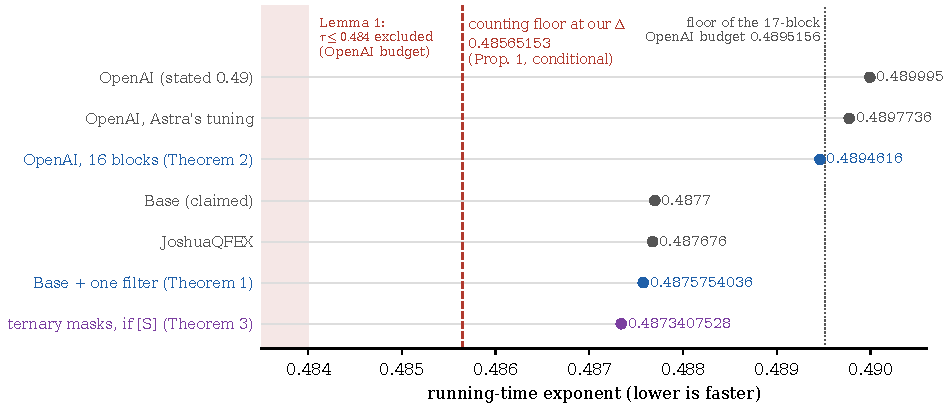
\includegraphics[width=\linewidth]{figures/fig_exponents.pdf}
\caption{Exponents discussed in this paper (lower is faster). Blue: this paper; purple: conditional on the open statement [S]; grey: other work. Theorems~1 and~2 have certified numerics and are conditional on the cited written proofs; Base's 0.4877 is its own claim. The dashed line is the counting floor of Proposition~\ref{prop:floor} at the checksum gap of Theorem~\ref{thm:main}, which applies to designs that enumerate every alias class; the dotted line is the floor of the 17-block OpenAI budget found in~\cite{astra}; the shaded band is excluded for the original OpenAI proof's budget by Lemma~1. Meet in the middle (0.5) and Li--Ye (0.4999978) lie off the scale.}
\label{fig:exponents}
\end{figure}

Base changes both the list construction and the estimator. In our tested density families and searches for the original construction (Sections~5--7), the best exponents remain near 0.4895. Combining Base's list construction with our asymmetric filter reaches threshold 0.4875754036 (Section~8). Section~9 distinguishes the costs at that point from a general limitation: under the enumeration and alias-class-count premises of Proposition~\ref{prop:floor}, retaining its checksum gap gives the lower bound $(1-\Delta)/2$.

The main contributions are the certified conditional theorem above; a first-moment obstruction for the original sufficient budget and an algebraic analysis of Base's costs; and a precise small-layer conjecture with a conditional ternary improvement and proved special cases. Supporting results include a certified 16-block point for the original OpenAI construction and an independent certification of the 430 moment premises used by the Base/JoshuaQFEX bound.

\subsection*{How to read this paper}
Section~2 introduces the model and notation. For the main result, continue to Section~8 (Base's construction, Corollary~D and the certified point), Section~9 (why the exponents stall) and Section~10 (the conditional extension and open problems). Section~3 audits the historical Base/JoshuaQFEX certificates; Sections~4--7 analyse the original OpenAI construction and its 16-block improvement. Section~11 gives the methods, verification ledger and AI disclosure. Appendix~\ref{app:T} states the ternary alias step, and Appendix~\ref{app:B} supplies the combinatorial proofs.


\paragraph{Reading the evidence labels.}
``Certified'' describes rigorous numerical inequalities; ``conditional'' describes dependence on the cited algorithmic proofs or an open conjecture. The two labels are compatible. Floating optimization is evidence, not proof. The claim-by-claim ledger in Section~11 separates these categories and records the remaining imported premises.


%======================================================================
\section{The OpenAI architecture and its parameter budget}

Throughout, running times are for randomized algorithms that answer correctly with probability at least $2/3$, in the word-RAM model of the OpenAI paper, on inputs whose integers and target have bit length $b \le n^c$ for an arbitrary fixed $c$; the constant in the $O(\cdot)$ depends on $c$. This is the setting of the OpenAI and Base theorems, and every bound below inherits it.

\textbf{Notation.} The symbols used throughout are collected here; each is explained again where it is first used.

\begin{center}
\small
\begin{tabularx}{\linewidth}{>{\raggedright\arraybackslash}p{4.4cm} L}
\toprule
Symbol & Meaning \\
\midrule
$n$; $b$ & number of input integers; largest bit length of the input integers and the target \\
$h(x) = -x\log_2 x - (1-x)\log_2(1-x)$ & binary entropy, with $h(0) = h(1) = 0$ \\
$\Sigma(B)$, $\Sigma_j(B)$ & the distinct subset sums of a set $B$ of input positions; those of its $j$-element subsets \\
$d(B) = |B| - \log_2|\Sigma(B)|$ & deficiency of $B$ (0 when all subset sums of $B$ are distinct) \\
$a_j(B) = |\Sigma_j(B)|/\binom{|B|}{j}$ & fraction of distinct values among the $j$-subset sums of $B$ \\
$P$, $\eta$ & the random checksum prime, of about $\eta n$ bits \\
alias; alias class & a subset whose sum agrees with the target modulo $P$ without being a solution; subsets that the list side cannot tell apart (in Base: equal on the shared block, with the same sums on each outside block) form a class, and a class consists of aliases entirely or not at all \\
$\tau$ ($\tau_0$ in Base); $T$ & exponent of the enumeration budget; final exponent threshold, the largest of the terms in the running-time formula below \\
$\Delta = \eta - \tau$, $\Gamma = 2\tau - \eta$, $a_\Gamma = \Delta/\Gamma$ & the checksum gap, its complement and their ratio \\
$M_1$, $M_2$; $p$, $q_m$ ($q$ in Base); $\kappa$ & the two filtering moments; their multipliers; the power applied to the densities \\
$\rho_c < \rho_f$ & the certified moment threshold and its finite-circle counterpart \\
OpenAI: $K$, $\mu = m/n$, $\gamma$, $d$, $d_0$, $d_1$, $c_0$, cap & number of disjoint half-blocks, block size, rate of the smaller modulus, local deficiency cutoff, preliminary-search thresholds, probability of a useful block, time cap \\
Base: $M, L, R$; $\mu$, $l$, $r = 1 - \mu - l$; $a$; $P'$; $\sigma = m/2$, $k \approx am$ & shared block and outside blocks; their sizes divided by $n$; mask density; the second, smaller random prime that filters representations (of rate $\gamma$); half-block size and mask size \\
$\eps$, $\zeta$; $g_0$; guard & small slack constants ($\eps = \zeta = 10^{-8}$ in Section~8); the guard margin $g_0 = 10^{-5}$ of the OpenAI budget; Base's input-length guard ($10^8$) \\
\bottomrule
\end{tabularx}
\end{center}

The algorithm's running time is $2^{(T+o(1))n}$ with $T = \max(\tau + 20\eps, \mathrm{cap}, \mu + 1/4, \eta/2)$. A parameter point is valid when the inequalities below hold. Here $\eta n$ is the bit length of a random prime $P$, $\tau n$ the list and enumeration budget, $\mu = m/n$ the shared block size, $\gamma$ the smaller-modulus rate, $d$ the local deficiency, $K$ the number of disjoint half-blocks (17 in the paper), $\eps = 10^{-8}$ and guard margin $g_0 = 10^{-5}$.

\begin{center}
\small
\begin{tabularx}{\linewidth}{>{\raggedright\arraybackslash}p{3.2cm} L >{\raggedright\arraybackslash}p{3.6cm}}
\toprule
Constraint & Inequality & Source (TeX) \\
\midrule
Block fit & $K\mu < 1$ & aliases l.79 \\
Filtered list & $\tau \ge 1/2 + (h(1/4) - 1/2 - \gamma)\mu$ & aliases l.201--211 \\
Visited pairs & $\tau \ge 1 + (2h(1/4) - 1 - \gamma)\mu - \eta + g_0$ & aliases l.244--253 \\
Sparse distinctions & $\eta > h(\mu) + \mu + g_0$ & aliases l.296--309 \\
Setup work & $T \ge \mu + 1/4$ & aliases l.163--169 \\
Many weights & $1/2 - d > \gamma$ & aliases l.354--399 \\
Useful block (Markov) & $1 - d_0/(K d \mu) > c_0 > 0$ & aliases l.336--352 \\
Preliminary search & $d_1 < d_0$, $\mathrm{cap} > 1/2 - d_1$ (strict) & setup l.157--219 \\
Trial division & $T > \eta/2$ & implementation l.283--285 \\
Checksum balance & $\Delta = \eta - \tau > 0$, $\Gamma = 2\tau - \eta > 0$ & checksum l.180--199 \\
Domination, case 1 & $1 \le p$, $3p \le 30$ & checksum l.443--449 \\
Domination, case 2 & $1 \le q_m$, $q_m(4a_\Gamma + 3) \le 30$, $a_\Gamma = \Delta/\Gamma$ & checksum l.451--458 \\
Error decay & $\rho_c < \rho_f < \eta - 48\eps$ & checksum l.487--495; filtering l.116--155 \\
Filtering moments & $M_1, M_2 < 2^{\rho_c}$ & filtering l.90--103 \\
\bottomrule
\end{tabularx}
\end{center}

The circle is $\mathbb T=\mathbb R/(2\pi\mathbb Z)$. All means and integrals below use normalized measure $dx/(2\pi)$; the notation $dx$ in circle integrals abbreviates this measure. All logarithms and relative entropies are in bits. For positive densities $f, g$ and $\kappa > 0$, with $K_x(w) = f(x+w)g(w)/Q(x)$ and $Q(x) = \mean_w f(x+w)g(w)$, the paper's scores are $u = A + E - D$ and $v = 2D - A - E$, where $D = \KL(K_x \,\|\, \mathrm{uniform})$, $A = \E_K \log_2 f^*(x+w)$, $E = \E_K \log_2 g^*(w)$, and $f^* = f^\kappa / \mean f^\kappa$ (likewise $g^*$).
\begin{gather*}
M_1 = \int_{\mathbb T} (2+2\cos x)\, 2^{\,p(\Delta - u(x))}\, dx, \qquad M_2 = \int_{\mathbb T} (2+2\cos x)\, 2^{\,q_m(a_\Gamma v(x) - u(x))}\, dx
\end{gather*}
The pair $(x, w)$ enters through $y - \theta = x + w$ (correlation, not convolution). With symmetric densities this convention is invisible; with asymmetric ones it matters (Section~7).

\paragraph{The filters used in the certificates.}
The coefficient arrays specify log-density polynomials, not densities themselves:
\begin{align*}
r(x)&=\sum_{j=1}^{16}\bigl(r_{c,j}\cos(jx)+r_{s,j}\sin(jx)\bigr),&
s(x)&=\sum_{j=1}^{16}\bigl(s_{c,j}\cos(jx)+s_{s,j}\sin(jx)\bigr),\\
f(x)&=\frac{2^{r(x)}}{\mean 2^r},&g(x)&=\frac{2^{s(x)}}{\mean 2^s}.
\end{align*}
In each candidate file, the first 16 entries of \texttt{rc} are $r_{c,j}$ and the next 16 are $r_{s,j}$, in increasing $j$; \texttt{sc} has the same ordering for $s$. Decimal strings are exact rational inputs. These formulas give strictly positive smooth densities. The scalar right-block fraction $r=1-\mu-l$ used in Base's list analysis is separate from the function $r(x)$.


%======================================================================
\section{Certifying the premises of the conditional 0.487676 bound}

All 430 continuous moment inequalities that the JoshuaQFEX bound assumes hold, certified twice. The tightest, filter 28 in region $\rho_0$, clears its assumed margin 0.00025 by $3.79\times10^{-6}$ in $\log_2$.

Each inequality has the form below, for filters $v = 0,\dots,42$ and regions $\rho_0,\dots,\rho_9$, with required margins 0.00025 ($\rho_0$, $\rho_1$), 4 ($\rho_2$--$\rho_8$) and 17 ($\rho_9$).
\begin{gather*}
I_b(v,\rho) = \int_{\mathbb T} (2+2\cos x)\, 2^{\,z\cdot G(x)}\, dx \;<\; 2^{\,\eta_b - m_\rho}, \qquad \eta_b = 0.51613
\end{gather*}
Here $z$ is the nonnegative multiplier vector supplied for that filter and region, and $m_\rho$ is the required margin above. To distinguish filter indices from the score $v(x)$, write Base's filter index as $j$. Its score $w_j$ is our second score $v_j$. With $b_0=1$, $b_1=1.25$, $b_2=1.6$, $b_3=2$, $b_4=2.6$, $b_5=3.5$, $b_6=5$, $b_7=8$, $b_8=15$, and a specified comparison set $C$, the rows of $G$ are
\[
\begin{cases}
(\Delta-u_j,\ \Gamma-v_j,\ (u_j-u_h)_{h\in C}),&\rho_0,\\
(a_\Gamma v_j-u_j,\ v_j-\Gamma b_{i-1},\ \Gamma b_i-v_j,\ (u_j-u_h)_{h\in C}),&\rho_i,\ 1\le i\le8,\\
(a_\Gamma v_j-u_j,\ v_j-15\Gamma,\ (u_j-u_h)_{h\in C}),&\rho_9.
\end{cases}
\]
The region fixes a band for the second score's type average. Base's Appendix~C supplies $z$ and $C$ for each row of the certificate inventory; the integral above tests that particular sufficient certificate.


\begin{itemize}
\item \textbf{Route A:} python-flint arb at 200 bits; analytic-strip trapezoid error bounds~\cite[Thm.~3.2]{tw} for the inner and outer quadratures; a strip bound on the integrand from a contour split, Cauchy--Schwarz and Parseval monotonicity. Outer error $1.8\times10^{-218}$.
\item \textbf{Route B:} an independently written mpmath interval implementation with different node counts and strip widths. It agrees with Route A to $< 5\times10^{-13}$ in $\log_2$ margin on 422 of 430 inequalities; the remaining 8 have looser but still passing enclosures.
\item \textbf{Least margins} reproduce Base \S8.2 to every printed digit: 0.000253791727569 ($\rho_0$), 0.000359513928220 ($\rho_1$), 4.15582444577 ($\rho_2$).
\item \textbf{The paper's own transferred certificates}, evaluated directly at $\tau = 0.48767595$ and $\eta = 0.51612858$, all exceed the required $10^{-6}$; the least is $1.3154\times10^{-4}$, about 48 times the paper's uniform worst case.
\item \textbf{Controls:} reproduction of earlier rigorous moments to $10^{-19}$; rejection of a false threshold and of a perturbed $\Delta$; doubled resolution identical to 15 digits.
\item \textbf{Exported decimals} use directed rounding (lower bounds rounded down, upper bounds up), verified in interval arithmetic.
\end{itemize}

\textbf{Scope.} This certifies the numerical premises of the bound. Its non-numerical premises (finite-circle convergence, the isolation and alias lemmas, and the word-RAM accounting) are those of the OpenAI and Base papers, which we take as given here; Section~10 lists their independent verification as an open task.

%======================================================================
\section{Changing the block count}

The constant 17 enters the OpenAI proof in two places, and both hold verbatim for any integer $K \ge 1$ with $K\mu < 1$ (the replacements below also need $\mu \le 1/2$, the range of the sparse-distinction count). Every other dependence on block size runs through $\mu = m/n$, and the checksum section is generic in $(\eta, \tau)$.

\begin{enumerate}
\item \textbf{Block fit (aliases l.79).} The paper needs $17 m/2 \le \lfloor n/2 \rfloor$; in general $K m/2 \le \lfloor n/2 \rfloor$, which holds for large $n$ when $K\mu < 1$.
\item \textbf{Partition and Markov (aliases l.336--352).} A uniform $\lfloor n/2 \rfloor$-set is partitioned into $K$ disjoint sets of size $m/2$, each with the law of $S$. Superadditivity and nonnegativity of deficiency give $K\, \E\, d(S) \le d_0 n$. Markov then gives $\Pr[d(S) \le d m] \ge 1 - d_0/(K d \mu) - o(1)$, which must exceed a fixed $c_0 > 0$. The later product $c_0/(m+1) \cdot 1/2 \cdot 1/(4 K_0 n^2) \ge n^{-4}$ holds for any fixed $c_0 > 0$.
\end{enumerate}

The remaining replacements are mechanical: 0.0567 becomes $\mu$ throughout, so the sparse-distinction count becomes $2^{(h(\mu)+\mu)n}$ (valid for $\mu \le 1/2$), the setup bound becomes $T \ge \mu + 1/4$, and $0.4894 > \gamma$ becomes $1/2 - d > \gamma$. In the checksum, the fixed 0.5168/0.5169 thresholds become $\rho_c < \rho_f < \eta - 48\eps$, and the error decay $2^{-0.0007n}$ becomes $2^{-(\eta - \rho_f - 48\eps)n}$, which still absorbs the $2^{O(\sqrt{n})}$ pattern count.

The constraints that do not depend on $K$ are isolation, the prime-collision lemma, the deficiency lemmas, alias subtraction and the word-RAM accounting. The old moment certificate does not transfer: new densities need a new numerical appendix (Section~7).

\textbf{Verification.} This section rests on a line-by-line reading of the OpenAI source; an independent reviewer re-derived the full constraint list from the \TeX{} and found nothing missing. The partition step (item~2) and the coupling with the preliminary search were verified by careful reading against the source; a fully written independent proof of these two steps is left to future work.

%======================================================================
\section{A lower bound on the first moment for all densities}

\begin{lemma}
For all strictly positive continuous densities $f, g$ on the circle, every $\kappa > 0$, $\Delta \ge 0$ and $p > 0$:
\begin{gather*}
\log_2 M_1 \;\ge\; \Phi(p) := 1 + p\,\Delta + (1+p)\log_2 \int_{\mathbb T} (1+\cos x)^{1/(1+p)}\,dx, \\ \int_{\mathbb T} (1+\cos x)^b\,dx = \frac{2^b\,\Gamma(b+\tfrac12)}{\sqrt{\pi}\;\Gamma(b+1)}
\end{gather*}
\end{lemma}

\begin{proof}
\leavevmode
\begin{enumerate}
\item \textbf{Jensen.} Since $K_x$ is a probability density in $w$, $u(x) = \E_K \log_2[f^*(x+w)\, g^*(w) / K_x(w)] \le \log_2 Q^*(x)$, where $Q^*(x) = \mean_w f^*(x+w)\, g^*(w)$. By shift invariance $Q^*$ is itself a probability density on the circle.
\item \textbf{Rewrite.} With $w(x) = 1 + \cos x$, also a probability density, $M_1 = 2^{1+p \Delta}\, \E_w[2^{-p u}] \ge 2^{1+p \Delta}\, \E_w[{Q^*}^{-p}]$.
\item \textbf{H\"older.} Write $w^{1/(1+p)} = (w\, {Q^*}^{-p})^{1/(1+p)}\, {Q^*}^{p/(1+p)}$ and use exponents $1+p$ and $(1+p)/p$. Since $\mean Q^* = 1$, $\E[w^{1/(1+p)}] \le (\E_w[{Q^*}^{-p}])^{1/(1+p)}$, which is the claim. \qedhere
\end{enumerate}
\end{proof}

\textbf{Tightness.} Equality in step 1 holds when the ratio $f^*(x+w)\,g^*(w)/K_x(w)$ is constant in $w$ under $K_x$ (for example when $\kappa = 1$, or when $f = g = 1$), and equality in step 3 needs $Q^*$ proportional to $w^{1/(1+p)}$. Densities with $g$ sharply peaked and $f$ proportional to $w^{1/(1+p)}$ approach the bound, with gaps down to $5.8\times10^{-7}$ in $\log_2$; in the family we tested, a positive gap remains at $\kappa = 1.1$. Write $\Psi(p) = (1+p) \log_2 \E[w^{1/(1+p)}]$, so that $\Phi(p) = 1 + p\Delta + \Psi(p)$. The function $\Psi$ is a log power mean of $w$ and is nonincreasing in $p$. On a cell $[p_L,p_R]$, $\Phi(p)\ge 1+p_L\Delta+\Psi(p_R)$; this gives rigorous cellwise lower bounds.

\textbf{Finite circle.} On $\mathbb{Z}/P\mathbb{Z}$ the same argument holds with the discrete average of $w^{1/(1+p)}$. For even $P$ that average is smaller than the closed form, so the closed form alone is false there (a reviewer's counterexample at $P = 4$ has gap $-0.154$; the gap shrinks roughly like $P^{-1-2/(1+p)}$). The algorithm uses $P \sim 2^{\eta n}$, so the correction is negligible, and the paper's premise is the continuous inequality anyway.

\textbf{Consequence 1: the eight-block point fails.} Astra's eight-block scalar point ($\eta = 0.67$, $\Delta = 0.1900002$) passes all twelve scalar inequalities. Lemma~1 gives $\log_2 M_1 \ge 0.885370$ for every $p$ in $[1, 10]$ (interval-evaluated on 9000 monotone cells), against the 0.669998 required: a shortfall of 0.215 bits for every possible filter.

\textbf{Consequence 2: the OpenAI budget cannot reach 0.48.} The sufficient conditions of the OpenAI proof include the $M_1$ condition with a multiplier $p \in [1, 10]$ (the rounding cap $3p \le 30$). Writing $\eta = \tau + \Delta$, Lemma~1 turns that condition into $(p - 1)\Delta < \tau - 1 - \Psi(p)$. At $p = 1$ this reads $\tau > 1 + \Psi(1) = 1 + 2\log_2(2\sqrt2/\pi) \approx 0.697$, which fails; for $p \in (1, 10]$ it forces $\Delta < D_{\max}(\tau)$ = max over $p$ of $(\tau - 1 - \Psi(p))/(p - 1)$, about 0.0403 at $\tau = 0.48$. The list bound forces $\mu \ge (1/2 - \tau)/(\gamma + 1/2 - h(1/4))$, and the pair bound with $\gamma < 1/2$ then forces $\Delta \ge 2.6494(1/2 - \tau) + g_0$, about 0.053 at $\tau = 0.48$. These constraints are jointly infeasible for every $\tau \le 0.484$, every $p \in [1, 10]$ and every $K$ (checked in interval arithmetic by two independent reviewers), so the sufficient conditions of the OpenAI proof cannot be met at exponent 0.48 for any choice of parameters. This is a statement about that proof's budget, not a lower bound for every algorithm built on related ideas. Combining Lemma~1 with the full scalar budget gives a sharper floor near 0.4852 ($K = 11$), but only as a floating, grid-based estimate.

\textbf{Verification.} An independent reviewer checked each step of the proof and found no counterexample in 300 random and 16 adversarial instances (minimum gaps $+0.107$ and $+0.0009$).

%======================================================================
\section{Working backward from 0.48 in the OpenAI construction}

OpenAI's paper proves exponent 0.49. Section~5 excludes 0.48 for that proof's sufficient conditions, for every parameter choice. The floating exploration below asks a finer question: what limits the best points found within this construction? In the density families and searches tested, joint moment capacity restricts the scalar budget to exponents near 0.4895. Section~8 obtains a lower exponent using Base's modified construction; these searches do not prove that every improvement must use that modification.

In these searches the binding resource is the joint capacity of the two moments: the largest $\Delta = \eta - \tau$ at which some densities keep both $M_1$ and $M_2$ below $2^\eta$. At $\tau = 0.4898$ that capacity is about 0.029 in every density family we tried (floating exploration).

\begin{center}
\small
\begin{tabularx}{\linewidth}{L >{\raggedright\arraybackslash}p{2.4cm} >{\raggedright\arraybackslash}p{2.0cm} L}
\toprule
Density family & Moments imposed & Capacity ($\Delta$) & What binds \\
\midrule
6 cosines (Astra's family) & $M_1$ and $M_2$ & 0.02810 & both moments \\
6 cos + 6 sin, $\kappa \in [0.5, 2]$ & $M_1$ and $M_2$ & 0.02841 & both moments \\
16 or 32 cos + sin, Astra-basin starts & $M_1$ and $M_2$ & 0.02864 & both moments \\
16 cos + 16 sin, random starts & $M_1$ and $M_2$ & 0.02908 & both moments \\
6 cosines & $M_2$ only & 0.03226 & rounding cap $q_m(4a_\Gamma+3) \le 30$ \\
6 cosines & $M_1$ only & 0.0396 & $M_1$ (Lemma~1 ceiling 0.0427) \\
\bottomrule
\end{tabularx}
\end{center}

Two observations from these floating searches follow.

\begin{itemize}
\item \textbf{Fewer blocks did not help in the tested searches.} With the tested density families and starts, each $K$ from 9 to 13 gave a worse best value than 17 (best 0.48978 at $K=13$). Along the tested continuations toward block size $1/K$ for $K=11,12$, $T$ increased while the moments kept $\Delta$ near 0.0284. These comparisons are not global optima over all densities.
\item \textbf{Each unit of capacity is worth about 0.35 in the exponent.} The floor of the audited budget, optimized over $K$, falls as capacity rises (floating, optimistic closure):
\end{itemize}

\begin{center}
\small
\begin{tabular}{lll}
\toprule
Joint capacity $\Delta$ & Floor on $T$ & Best $K$ \\
\midrule
0.0281 (the 6-term family) & 0.48977 & 17 \\
0.032 & 0.48840 & 15 \\
0.036 & 0.48703 & 13 \\
0.0396 ($M_1$'s own capacity) & 0.48579 & 12 \\
\bottomrule
\end{tabular}
\end{center}

At the current capacity this reproduces Astra's certified basin, which is the control. A further 0.001 of capacity, which richer asymmetric densities do supply, already moves the best $K$ from 17 to 16; Section~7 certifies that point.

%======================================================================
\section{A certified 16-block point at 0.4894616}

\begin{theorem}[conditional on the OpenAI proof and Section~4]\label{thm:k16}
With the parameters below, the OpenAI algorithm (randomized, word-RAM, inputs of bit length at most $n^c$ for any fixed $c$) decides Subset Sum in time $O(2^{T' n})$ for every $T' > 0.4894615727$, in particular $O(2^{0.4894616 n})$.
\end{theorem}

\begin{center}
\small
\begin{tabularx}{\linewidth}{>{\raggedright\arraybackslash}p{3.3cm} L >{\raggedright\arraybackslash}p{3.6cm}}
\toprule
Parameter & Value & Replaces \\
\midrule
Half-blocks $K$ & 16 & 17 \\
Block size $\mu$ & 0.0593373017 & 0.0567 \\
$\eta$ & 0.5184804040 & 0.51772 \\
$\tau$ & 0.4894613727 & 0.48996 \\
$\gamma$ & 0.4888978551 & 0.48925 \\
$\kappa$ & 1.03489429 & 1.0315 \\
$p$, $q_m$ & 8.38520435, 8.19573911 & 8.5, 8.3 \\
Log-density polynomials $r$, $s$ & 16 cosine + 16 sine terms each (64 coefficients, 8 decimals) & 6 cosine terms \\
Coverage constant $c_0$ & 0.0001 & 0.005 \\
$d$, $d_0$, $d_1$ & $1/2 - \gamma - 10^{-8}$; $(1-c_0)K d \mu (1-10^{-7})$; $d_0 - 10^{-9}$ & 0.0106, 0.01004, 0.010025 \\
cap; $\rho_f$; $\rho_c$ & $\tau + 20\eps$; $\eta - 48\eps - 5\times10^{-7}$; $\rho_f - 10^{-6}$ & 0.489985; 0.5169; 0.5168 \\
\bottomrule
\end{tabularx}
\end{center}

The exact coefficients are in \texttt{candidate\_K16.json} in the repository (Section~11).

\textbf{Certificates.}

\begin{itemize}
\item \textbf{Ours} (python-flint arb, 200 bits): inner trapezoid with $N_{\mathrm{in}} = 256$ on a strip of half-width 0.3, outer $N = 8192$ on a strip of half-width 0.2. $q_0 = 0.372$, so $\log_2 Q$ is analytic on the strip. Quadrature errors are below $10^{-27}$. Result: $\log_2 M_1 \approx 0.518477576190$ and $\log_2 M_2 \approx 0.518477347232$, against $\rho_c = 0.5184784240$. All 20 interval margins are positive; the moment margins are $8.48\times10^{-7}$ and $1.08\times10^{-6}$. Doubled resolution agrees to 20 digits.
\item \textbf{Independent check:} an independently derived condition list and an interval DFT evaluation, including aliasing and tail bounds, give agreement to 16 digits. The provenance and exposure qualifications are recorded in Section~11.
\item \textbf{Controls:} the same certifier passes Astra's certified 17-block point below its own threshold and rejects that point with $\Delta$ raised by 0.001.
\end{itemize}

\textbf{Conventions the result depends on.}

\begin{itemize}
\item \textbf{Orientation.} The densities are asymmetric, so the correlation convention $y - \theta = x + w$ ($Q(x) = \mean_w f(x+w)g(w)$) is load-bearing. Reflecting one density gives $\log_2 M \sim 3.28$, a catastrophic failure. Swapping $f$ and $g$, or $x \to -x$, is harmless because the weight is even.
\item \textbf{Admissibility.} filtering.tex l.16 allows any strictly positive continuous densities; nothing in the proof uses symmetry. The old numerical appendix used the $j \leftrightarrow 64-j$ symmetry and is replaced by either certifier.
\item \textbf{Thin slacks.} Several margins are $10^{-9}$ to $10^{-6}$. They only make the cutoff $n_*$ astronomically large: Chebyshev with $d_0 - d_1 = 10^{-9}$ makes the preliminary-search bound meaningful only for $n$ of order $10^{18}$ or more. Nothing fails asymptotically.
\end{itemize}

At $\mu = 0.0593 > 1/17$, seventeen blocks would not fit: the gain comes from trading one block for a larger shared block, which the extra moment capacity of the new densities pays for.

%======================================================================
\section{Below JoshuaQFEX: Base's construction with one asymmetric filter}

Base changes both halves of the OpenAI algorithm. On the list side it partitions the input into a shared block $M$ of about $0.475n$ positions and two outside blocks $L$ and $R$, uses sparse masks of density $a \approx 0.008$, returns alias phase sums instead of alias lists, and replaces the 17-block Markov step by an averaged small-layer bound, Base's Corollary~D. On the checksum side it uses a family of 43 filters, each with 8 cosine terms, certified in 10 regions of the pattern space. Base reports that its filter search stalls near 0.4876 and that ``further progress needs a new idea.'' JoshuaQFEX retunes Base's parameters to 0.487676.

\textbf{Why Corollary D is needed.} A trial of Base's alias step uses a random half $S$ of $M$ and looks for representations of an alias through $k$-element subsets of $S$, with $k \approx am$. Repeating trials helps only if these subsets produce enough distinct sums, and Corollary D supplies the averaged lower bound:

\begin{quote}
\textbf{Corollary D} (Base, l.254--257). Let $k, \sigma, v$ be nonnegative integers with $2k \le \sigma$, $2\sigma \le v + 2k$, $v \le |M|$ and $\binom{\sigma}{k}\binom{v}{k} \le 2^v$. Let $S$ be a uniform $\sigma$-subset and $V$ a uniform $v$-subset of $M$. Then $\E_S\, a_k(S) \ge \E_V\, 2^{-d(V)}/(v+1)$.
\end{quote}

In the alias step $\sigma = m/2$ and $v = m - 2k$, so $2\sigma = v + 2k$; write $g_M = -\log_2 \E_V 2^{-d(V)}$. So a random half-block has, on average, at least a $2^{-g_M}/(v+1)$ fraction of distinct $k$-subset sums. Base estimates $2^{g_M}$ by sampling and runs about $n^7\, 2^{g_M + O(n^{0.6})}$ trials. Each trial finds the class of a given alias with probability at least $2^{-g_M} n^{-6}$ (Base's Lemma A5), using the second prime $P'$ to keep many of the distinct sums in one residue class, so every alias class is found with high probability; Base's deficiency bounds keep the number of trials within the time budget. The numerical side conditions this needs are among Base's (C1)--(C8) and (S1)--(S5), certified below.

\textbf{Observation.} With a family of $J = 1$ filters, Base's Theorem B certificates collapse to OpenAI's two moments: region $\rho_0$ uses the multiplier vector $z = (p, 0)$, the bounded regions $\rho_1$--$\rho_8$ use $z = (q, 0, 0)$ and the unbounded region $\rho_9$, which has one row fewer, uses $z = (q, 0)$; all high regions share the exponent $q(a_\Gamma v - u)$, so the 10 certificates reduce to $M_1$ and $M_2$. Our asymmetric filters (Section~7) therefore drop into Base's construction unchanged, and Base's 43-filter family has to compete with one filter that carries sine terms and 16 harmonics.

\textbf{Price, then optimization.} In Base's alias budget each $+0.001$ of moment capacity lowers $\tau_0$ by about 0.00039 (control: zero extra capacity recovers 0.4876826, within $7\times10^{-6}$ of JoshuaQFEX). We then optimized Base's alias parameters ($\eta$, $\mu$, $a$, $\gamma$, $l$), one filter (16 cosine + 16 sine terms per density, and $\kappa$) and the multipliers $p$, $q$ jointly, under all of Base's alias constraints and both moment constraints. Four of four starts reached $\tau_0 = 0.4875749$, matching the pre-registered prediction $0.48757 \pm 0.0001$.

\textbf{The frozen point} (exact decimals, in \texttt{candidate\_base.json}):

\begin{center}
\small
\begin{tabular}{ll}
\toprule
Parameter & Value \\
\midrule
$\tau_0$ & 0.4875752036 \\
$\eta$ & 0.5162721413 \\
$\mu$ & 0.4752421539 \\
$a$ & 0.0082379228 \\
$\gamma$ & 0.0605824120 \\
$l$ & 0.4836347962 \\
$\kappa$, $p$, $q_m$ & 1.03465831, 8.45902160, 8.27015425 \\
$\eps$, $\zeta$, input guard & $10^{-8}$, $10^{-8}$, $10^{8}$ \\
$\rho_f$, $\rho_c$ & $\eta - 1.5\times10^{-6}$, $\rho_f - 10^{-6}$ \\
exponent $T = \tau_0 + 20\eps$ & 0.4875754036 \\
\bottomrule
\end{tabular}
\end{center}

\textbf{Certificate.} All 33 conditions (34 checks; our certifier also tests an implied one) were checked in ball arithmetic (python-flint arb, 200 bits) and all margins are positive: Base's alias constraints C1--C8, the size conditions S1--S5, Lemma A5 ($1/2 - \tau_0 + \zeta < \delta$), the Lemma A7 conditions, the Theorem A cap $1/\mathrm{guard} + \zeta < \eps_0$, the prime draw $\eta/2 < \tau_0$ (enough primes of that size by~\cite[Cor.~3]{rs}, as in~\cite{openai}), the Lemma B1--B3 bookkeeping, and both moments. The tightest margins are B3 ($8.1\times10^{-7}$), $M_1$ ($1.315\times10^{-6}$), C4 ($1.3156\times10^{-6}$) and $M_2$ ($1.494\times10^{-6}$). The moments are $\log_2 M_1\approx0.51626832585128515$ and $\log_2 M_2\approx0.51626814726466969$, rounded here for display. The full-precision stored balls have rigorous radii below $10^{-20}$; doubled quadrature resolution agrees to 20 digits.

\textbf{Independent checks and admissibility.} Independently derived condition lists and rigorous moment evaluators confirm the point; Section~11 records their provenance. The checks include Lemma A7 items 1, 3 and 4, S2, S5, the prime draw and $a_\Gamma\le3/4$, required for Base's Lemma B2 row error. Sine terms preserve strict positivity, smoothness and the relative-entropy identities. For the displayed log-density polynomials, summing harmonic amplitudes gives the safe bounds $|r(x)|,|s(x)|<3.21$; every required fixed derivative is bounded explicitly by the corresponding coefficient sum with harmonic powers. Thus the uniform-boundedness argument of OpenAI's Lemma 3.2 applies without an evenness assumption. The stored certificates, rather than rounded displays, carry the numerical error bounds.

\textbf{A conditional improvement to 0.4873408.} Section~9 describes ternary left masks: $k_1$ entries $+1$ inside the alias's half-block $S$ and $k_2$ entries $-1$ outside it, with a plain right mask and the expansion rule ``$X^+$ disjoint from $Y$, $X^-$ contained in $Y$''. A full replacement for Base's alias step in Base's style (soundness, counts, an explicit integer trial count of order $C_S\, n^8\, 2^{d(M)}$, a global distinctness lemma in place of Base's $\delta$, coverage through the counting identity of Section~10, and the cost items, with Base line numbers) is stated in Appendix~\ref{app:T}; its complete proofs are in the ancillary file and the repository (``Section~T''). The trial count carries the polynomial constant $C_S$ of [S] below, which does not change the exponent. At the optimum, frozen as $\tau_0 = 0.4873405528$, $\eta = 0.5159974155$, $\mu = 0.4746795055$, $a = 0.0035141538$, $c = 0.0035141537$, $\gamma = 0.0603737099$, $l = 0.4840025845$ with one 16 + 16 filter, all 33 conditions hold in arb at 200 bits (tightest margin $8.1\times10^{-7}$; $\log_2 M_1\approx0.51599187405865779$, $\log_2 M_2\approx0.51599162047014794$). Independent condition extraction and interval quadrature, with analytic error bounds, confirm the frozen point. Section~11 records the proof checks and numerical provenance; Appendix~\ref{app:T} and the accompanying Section~T text state the repaired procedure.

Here [S] (``small slices are robust'') is the statement: there is a polynomial $C_S$ such that for every integer weighting of an $m$-element block $M$ and every $k \le 0.11m$, $a_k(M) \ge 2^{-d(M)}/C_S(m)$, where $a_k(M)$ is the fraction of distinct values among the $k$-element subset sums and $2^{-d(M)}$ is the fraction of distinct values among all subset sums (Section~10).

\begin{theorem}[conditional on {[S]}, on Base's written proof and on the OpenAI paper]\label{thm:ternary}
Subset Sum can be solved by a randomized word-RAM algorithm, on inputs of bit length at most $n^c$ for any fixed $c$, in time $O(2^{T' n})$ for every $T' > 0.4873407528$, in particular in time $O(2^{0.4873408n})$.
\end{theorem}

This is $2.34\times10^{-4}$ below the point above and $3.35\times10^{-4}$ below JoshuaQFEX. We present it as conditional until [S] is proved. [S] is open; Section~10 reduces it to a sharper, purely combinatorial statement and gives the evidence for it.

\textbf{Status and caveats.} The exponent of Theorem~\ref{thm:main} is $T = \tau_0 + 20\eps = 0.4875754036$, so, in the setting of Section~2, the algorithm runs in time $O(2^{T' n})$ for every $T' > T$, in particular $O(2^{0.4875755n})$; $T$ is $1.005\times10^{-4}$ below JoshuaQFEX and $1.14\times10^{-4}$ below Base's $\tau_0$. It is conditional on Base's written proof (its alias-step cost accounting, Lemma A5 and its checksum changes) and on the OpenAI paper, exactly as JoshuaQFEX is. The constants $\zeta$ and the input guard are free in Base; our choices $\zeta=10^{-8}$ and $\mathrm{guard}=10^8$ only raise the cutoff $n$ beyond which the bound applies: Base's Proposition P then needs $n > 10^8$, and its Chebyshev term $4/(\zeta^2 n)$ is small only for $n$ of order $10^{17}$. Using our point in Base's proof changes some of Base's stated numerical constants, all of which remain valid: $\delta\approx0.0698$ (Base: $> 0.0706$; still far above the 0.0124 it is compared with), S3's left side $0.12946$ (Base: 0.129), $\eps_0 \ge 1.3156\times10^{-6}$ (Base $5.37\times10^{-6}$), the guard constant $10^8$, $c_z = 6p \approx 50.8$ (Base $\le 2511$) and the B3 error exponent $8.1\times10^{-7}$ (Base 0.00017). The OpenAI rounding caps $3p \le 30$ and $q(4a_\Gamma + 3) \le 30$ are not required under Base, whose Lemma B2 accounts for rounding through $6\eps\Sigma z$; they hold anyway. Base's filter definition and verification script assume cosine-only filters and need the corresponding extension to sine terms; the affected lines are listed in the repository.

%======================================================================
\section{Why the exponents stall near 0.4876}

This section analyses Base's parameter budget at the Section~8 point. The three closed forms are proved algebraic consequences of (C1)--(C8), and Proposition~\ref{prop:floor} is a counting implication under its explicit premises. Evaluation at the frozen point uses its exact decimal parameters. The re-optimizations, sensitivities and negative results are floating evidence from pre-registered experiments C13--C17; they do not establish global optima.

\textbf{Local sensitivities (floating evidence).} The following values report the estimated exponent saving per unit relaxation of a constraint near the optimized point, with the filter and other parameters allowed to vary. They describe local sensitivity, not the result of a finite one-bit relaxation:

\begin{center}
\small
\begin{tabularx}{\linewidth}{>{\raggedright\arraybackslash}p{2.2cm} L >{\raggedright\arraybackslash}p{4.2cm}}
\toprule
Constraint & What it counts & Exponent saved per bit \\
\midrule
C4 & matching visits & 0.389 \\
C1 & small prime $P'$ against the number of representations & 0.258 \\
C2 & left records & 0.077 \\
C3 & right class records & 0.077 \\
C5 & right masks times trials & 0.001 \\
$M_1$, $M_2$ & checksum moments, per bit of $\log_2 M$ & 0.051 \\
\bottomrule
\end{tabularx}
\end{center}

The entries identify the list constraints as the largest local sensitivities. They are not a decomposition of the running-time exponent. Interpreting them as KKT multipliers also requires the constraint normalization and stationarity residuals of the optimization run; the table is used here only as exploratory guidance.

\textbf{Three closed-form bounds.} Write $\eta = \tau_0 + \Delta$, where $\Delta$ is the gap the checksum allows, and use $l + r = 1 - \mu$. Adding C2 and C3, and rearranging C4 and C5, gives

\begin{itemize}
\item[(i)] $\tau_0 > 1/2 - \mu(\gamma - h(a)/2)$, from left records times right classes, where more representations help;
\item[(ii)] $2\tau_0 > 1 - \Delta + \mu[(h(a) - \gamma) + (h(1/2 - a) - 1)]$, from the matching visits together with the checksum, where smaller masks help;
\item[(iii)] $\tau_0 > (1/2 + \mu h(1/2 - a))/2$, from the right masks times the number of trials.
\end{itemize}

At the floating optimum behind our Section~8 point the three right sides are 0.4875739, 0.4875744 and 0.4875744, against $\tau_0 = 0.4875749$ (the gap is the $10^{-6}$ slack we imposed). At the frozen, certified point they are 0.4875739, 0.4875745 and 0.4875745 against $\tau_0 = 0.4875752$: (ii) and (iii) bind, and (i) sits $6.6\times10^{-7}$ lower. Our point and Base's are therefore a balance of these bounds. Bound (i) wants a larger mask fraction $a$, because $\gamma \le h(2a)/2$ grows faster than $h(a)/2$; bound (ii) wants a smaller one; bound (iii) holds the block size $\mu$ in place.

\textbf{The counting floor.} In (ii), $1 - \eta$ is $\log_2$ of $2^n/P$, the typical number of aliases of a target. This gives a floor for the alias-enumeration phase, under an explicit premise.

\begin{proposition}[counting floor]\label{prop:floor}
Consider an alias step that inserts every alias class of each target, spends at least one counted step on each class it inserts, and is combined with a checksum at the same modulus whose capacity is $\Delta$, so that $\eta - \tau_0 \le \Delta$. If for some input and target there are at least $2^{(1-\eta-o(1))n}$ alias classes, then $\tau_0 \ge 1 - \eta - o(1) \ge 1 - \tau_0 - \Delta - o(1)$, that is, $\tau_0 \ge (1-\Delta)/2 - o(1)$.
\end{proposition}

The premise concerns the input; the method does not supply it. Distinct subset sums alone do not imply it: the weights $P, 2P, 4P, \dots$ have distinct subset sums but no aliases of a target $\equiv 1 \pmod P$. Inputs whose subset sums spread nearly evenly over the residues modulo $P$, as one expects for typical random inputs, have about $2^{(1-\eta)n}$ aliases per target, each its own class when the subset sums are distinct. The proposition says nothing about designs that do not enumerate every alias class, that use different moduli, or whose checksum is not of the moment form, and it is not a lower bound for Subset Sum. At the frozen point, $\Delta=0.0286969377$ and $(1-\Delta)/2=0.48565153115$ exactly; Figure~\ref{fig:floor} shows the floor as a function of $\Delta$. This evaluation is distinct from the empirical observation that about 0.029 is the best joint capacity found in the searches of Section~6; no global maximum has been proved. Exponent 0.48 would need $\Delta \ge 0.040$ even with no list overhead at all; Lemma~1 caps the first moment's capacity near that value. The floor is attained in the model when the overhead in (ii) is removed. The table re-optimizes the filter at each step, so $\Delta$ drifts to 0.0284 and the floor it reaches is 0.4858; with the filter held fixed, the second reviewer's model gives 0.4875741, 0.4871563, 0.4867011, 0.4862020 and 0.4856515.

\begin{center}
\small
\begin{tabular}{ll}
\toprule
Share of the C4 overhead removed & $\tau_0$ \\
\midrule
none (Section~8 point) & 0.4875749 \\
25\% & 0.4871858 \\
50\% & 0.4867641 \\
75\% & 0.4863049 \\
all & $0.4858019 = (1 - \Delta)/2$ \\
\bottomrule
\end{tabular}
\end{center}

\begin{figure}[t]
\centering
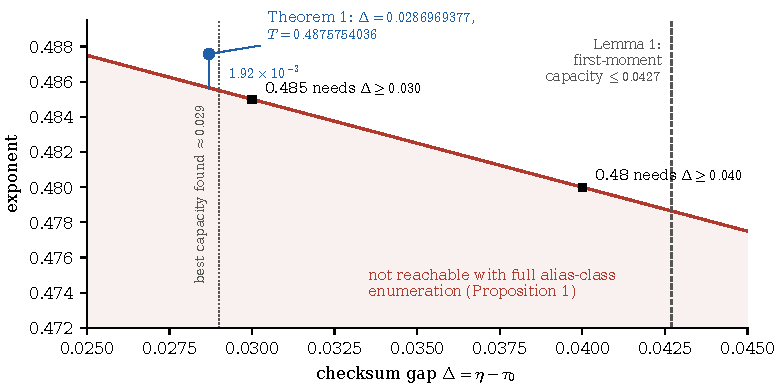
\includegraphics[width=0.82\linewidth]{figures/fig_floor.pdf}
\caption{The counting floor $(1-\Delta)/2$ of Proposition~\ref{prop:floor} against the checksum gap $\Delta$, under its enumeration and alias-class-count premises. The point of Theorem~\ref{thm:main} lies $1.92\times10^{-3}$ above the floor at its own gap. Reaching 0.485 with full enumeration needs $\Delta \ge 0.030$, and 0.48 needs $\Delta \ge 0.040$. The dotted line marks the best joint capacity found in our searches (about 0.029, floating evidence; Section~6); the dashed line is the bound on first-moment capacity from Lemma~1 (0.0427).}
\label{fig:floor}
\end{figure}

\textbf{What the overhead is.} The rest of (ii) is $\mu[(h(a) - \gamma) + (h(1/2 - a) - 1)]\approx0.003846$ per $n$ at our point. The probability that a uniform left mask of $k$ elements and a uniform right mask of $\sigma - k$ elements of the block are disjoint has $-\log_2$ equal to $\mu[h(a) + h(1/2 - a) - 1 - h(2a)/2]\,n + O(\log n)$, 0.003845 per $n$. The two differ by $\mu(h(2a)/2 - \gamma)$, which is $\mu$ times the slack of C1, about $6.3\times10^{-7}$ at our point; they agree in the limit $\gamma = h(2a)/2$. So, up to that slack, the overhead is the visited tuples with overlapping masks, which the expansion step tests and discards. It costs about one bit per left-mask element, because each element of a left mask lies in the alias's half-block $S$ with probability $1/2$.

\textbf{A restricted colour-coding model.} We tested the use of colour-coding~\cite{ayz} that confines left masks to a random region $R$ of size $\rho m$, while $S$ covers half of $R$. For fixed $\rho>0$ and small $a$, the left-mask contribution is $a+a^2/(2\rho\ln2)+O(a^3)$; the right-mask term is $h(1/2-a)-1=-2a^2/\ln2+O(a^4)$. The leading terms favour $\rho=1$. In the tested full-model optimizations, the exponent was worse by $1.4\times10^{-4}$ at $\rho=0.75$, $4.0\times10^{-4}$ at 0.5 and $1.2\times10^{-3}$ at 0.25. These calculations rule out an improvement in those tested configurations, not all uses of colour-coding. They motivate investigating representations that use information about $S$ or a different source of representations.

\textbf{Ternary masks need a stronger Corollary D} (the small-layer bound described in Section~8). Following the representation technique of Howgrave-Graham and Joux~\cite{hgj} and its ternary refinement by Becker, Coron and Joux~\cite{bcj}, let the left mask also carry $-1$ entries outside $S$. On the block outside $S$ the trial's signed weights are the negatives of the alias's own signing, so these entries add plain subset sums of that signing. In the floating model this reaches $\tau_0 = 0.4873403$, $2.35\times10^{-4}$ below our point, from four of four starts; the optimum splits Base's representations evenly between inside and outside $S$. The model assumes that Base's Corollary D holds for this two-part family essentially without loss. Losing 10\% of the outside representations removes the gain entirely, and the break-even is about 2\%. Base's proof of Corollary D starts from a layer $t \le v/2$ where many sums are distinct and descends to layer $k$ by a covering argument, which limits the support of the representations to $m/2 + k$. Under that limit a ternary mask with fractions $(a, c)$ is no better, in every constraint, than Base's own mask with fraction $a + c$. Under Base's Corollary D we therefore count ternary masks as a negative result. Under the stronger statement [S] of Section~8 they give Theorem~\ref{thm:ternary} ($T = 0.4873407528$); [S] is open (Section~10).

\textbf{The filter families we tested add almost nothing.} We tested families of two and three asymmetric filters in Base's format, with its comparison rows $u_v - u_l$. Base's own family is worth about $6.4\times10^{-4}$ bits of moment margin over its best single filter, which sets the scale. On top of our filter, the best two-filter family the optimizer found pairs the filter with its mirror image $x \to -x$, which covers the mirror of the filter's own critical type: $6.7\times10^{-5}$ bits of margin, lowering the exponent by only $3.3\times10^{-6}$. Twelve random second filters reach either that pair or nothing, and a third filter adds $4.6\times10^{-6}$ bits. In these tests, asymmetry and family diversity buy largely the same thing; larger or differently structured families remain untested. We did not certify the $3\times10^{-6}$ improvement.

Under Proposition~\ref{prop:floor}'s enumeration and alias-class-count premises, fixing the checksum gap at our certified value gives the lower bound $0.48565153115$. This leaves $1.92\times10^{-3}$ between that floor and the certified threshold; removing all of the C4 overhead in the model of the table above recovers about $1.77\times10^{-3}$ of it. The tested filter families, ternary masks under Base's Corollary~D, and restricted colour-coding model did not remove that distance. The floor is a proved conditional implication; the claims about those searches are floating evidence.

%======================================================================
\section{Open problems}

The central open problem on the checksum side is to prove an upper bound on the joint capacity of the two moments. Every density family we optimized stalls near $\Delta \approx 0.029$. A theorem showing that this is optimal for the moment format, or a family that exceeds it, would settle how far this architecture can go.

\textbf{Beyond the fixed-gap counting bound.} Under the enumeration and alias-class-count premises of Proposition~\ref{prop:floor}, retaining the checksum gap of our certified point gives the lower bound $(1-\Delta)/2$. Progress below that bound would require leaving at least one premise, for example by increasing checksum capacity or avoiding full alias-class enumeration. Two narrower questions remain on the list side.

\begin{itemize}
\item \emph{Corollary D beyond the half-block.} Let $S$ be a uniform half of the block and consider the family $\{U : |U \cap S| = k_1,\ |U \setminus S| = k_2\}$. Is the average fraction of distinct sums $w(U)$ at least $2^{-g_M}/\poly(n)$, with $g_M$ inside the trial budget (at most $d(L)$, $d(M)$ and $(1/2 - \tau_0 + \zeta)n$)? Within the support $m/2 + k$ this follows from Base's proof. Beyond it, a sumset argument is the natural attempt: a sum of two pieces can collapse only if both pieces are structured, and structure costs deficiency. Essentially lossless, the lemma is worth about $2.34\times10^{-4}$ through ternary masks. A cleaner sufficient statement exists. On the block outside $S$ the trial's signed weights are the negatives of the alias's own signing, so the family's sums are plain $k'$-subset sums ($k' = k_1 + k_2$) of one fixed signing, and a counting identity gives $\E_S[\text{fraction of distinct sums}] \ge a_{k'}(M)$, the fraction of distinct $k'$-subset sums of the whole block. So it suffices that small layers are robust, which is the statement [S] of Section~8; the subsection below reduces it to a chain of purely combinatorial statements and records what is proved.
\item \emph{A different source of representations.} The overlap waste of Section~9 is intrinsic to representations drawn from a uniform half $S$. Information about $S$ might reduce that waste; removing it entirely would be worth up to $1.77\times10^{-3}$, the full overhead measured in Section~9.
\end{itemize}

\subsection*{The small-layer statement [S] behind the conditional exponent}

Theorem~\ref{thm:ternary} needs [S] only at $k' = k_1 + k_2 \approx 0.0070m$; Section~8 states it for $k \le 0.11m$ because that is the range reached by the reduction below. Base's Corollary D and its size conditions are then not needed, and its cost bounds still hold if $\mu < l$. Write $s_j$ for the number of distinct $j$-subset sums of the block and $a_j = s_j/\binom{m}{j}$, and call a weighting \emph{generic} if, for each $j$, all its $j$-subset sums are distinct. The statements below are linked by
\[
\text{YP-Hall} \;\Rightarrow\; \text{Conj.~Q} \;\Rightarrow\; \text{Conj.~M}' \ (P = 1) \;\Rightarrow\; \text{[S]} \ (C_S = 3),
\]
In Conjecture M$'$, one fixed polynomial $P$ must work for every $m$, every integer weighting, and all integers $0\le k\le0.11m$ and $k\le t\le m-k$; $P$ is independent of the weighting and of $k,t$. The first implication covers $k\le m/4$, the second uses complementation, and the last is Lemma~S. The table gives the status of each link and of the partial results; proofs are in Appendix~\ref{app:B}.

\begin{center}
\small
\begin{tabularx}{\linewidth}{>{\raggedright\arraybackslash}p{2.6cm} L >{\raggedright\arraybackslash}p{4.7cm}}
\toprule
Statement & Content & Status \\
\midrule
{[S]} & $a_k \ge 2^{-d(M)}/C_S(m)$ for every weighting and $k \le 0.11m$ & Open; $a_k\,2^{d(M)} \ge 1.00$ in all 2,655 tested instances ($m = 12$ to $16$) \\
{Lemma S} & M$'$ with constant $P(m)$ implies [S] with $C_S = P + 2$ & Proved \\
{Conjecture M$'$} & $a_t \le P(m)\, a_k$ for $t \in [k, m-k]$, $k \le 0.11m$ & Open; proved with a loss of about $2^k$ (Proposition~\ref{prop:p2}) \\
{Conjecture Q} & $Q_w(t,k) \le 1$ for $k \le m/4$; implies M$'$ with $P = 1$ & Open; no violation for $k < m/3$ in our searches; false at $k = m/3$ \\
{YP-Hall} & a Hall condition for $t + 2k \le m$; implies Conjecture Q & Open; feasible in about 35,700 floating-point flow computations \\
{Case $k = 1$ of Q} & $Q_w(t,1) \le 1$ & Proved for $t = 2$ and for two families of weights (Proposition~\ref{prop:k1}); open for $t \ge 3$ \\
{Exact monotonicity} & $a_{k+1} \le a_k$ for $k + 1 \le m/2$ & False at the middle step (130 counterexamples at $m = 8$); not needed \\
\bottomrule
\end{tabularx}
\end{center}

\emph{Lemma S.} If $a_t \le P(m)\, a_k$ for all $t \in [k, m-k]$ and $k \le 0.11m$, then [S] holds with $C_S = P + 2$. Indeed $2^{-d(M)} \le \E_{t\sim\mathrm{Bin}(m,1/2)}[a_t]$, since $|\Sigma| \le \sum_t |\Sigma_t|$; the layers inside $[k, m-k]$ contribute at most $P a_k$, and the layers outside carry mass at most $2\cdot 2^{-m(1-h(\alpha))}$ with $\alpha = k/m$, which is at most $2a_k$ because $a_k \ge 1/\binom{m}{k} \ge 2^{-mh(\alpha)}$ and $h(\alpha) \le 1/2$ for $\alpha \le 0.11$. (At $k = 0$ there are no outside layers.)

\emph{Exact monotonicity fails at the middle step.} An exhaustive sweep over all value multisets in $[-8, 8]$ at $m = 8$ finds 130 counterexamples to $a_{k+1} \le a_k$, all at the middle step $k + 1 = m/2$, for example $w = (-6, -5, -5, -3, -3, -2, 4, 5)$ with $a_3 = 19/56 < a_4 = 24/70$ (verified independently). Away from the middle the comparison held in our tests: in exhaustive sweeps at $m = 9$ to 12 (about 11 million multisets) the maximum of $a_t$ over $t \ge k$ was attained at $t = k$ for every $k \le m/4$. The tight cases are sharp: with half the weights equal to 1 and half to 2, $a_k/a_{k+1} = (m - k)/(k + 2)$, exactly 1 at $k = m/2 - 1$. Monotonicity also has an exact combinatorial form: the map $(y, e) \mapsto (e, y - w_e)$ is a bijection between pairs with $y$ a $(k+1)$-sum and $e$ in the union $U(y)$ of its witness sets, and pairs with $x$ a $k$-sum and $e$ outside the intersection $C(x)$ of its witness sets, so $a_k \ge a_{k+1}$ is equivalent to $\sum_y (|U(y)| - (k+1)) \ge \sum_x (k - |C(x)|)$ (verified on 39 instances).

\begin{proposition}[P2]\label{prop:p2}
For $k \le t \le m - k$, $s_t\binom{t}{k} \le s_k\binom{m}{t-k}$, that is, $a_t \le a_k\,\binom{m}{t-k}\big/\binom{m-k}{t-k}$.
\end{proposition}
Fix one witness $X_y$ for each $t$-sum $y$; the map $(y, A) \mapsto (w(A), X_y \setminus A)$ over $k$-subsets $A \subseteq X_y$ is injective, because the image determines $y$, hence $X_y$, hence $A$. The loss is about $2^k$ at $t = m/2$; it is exactly the support barrier $m/2 + k$ of Base's Corollary D seen as a statement about layers. At $k = 0.007m$ it costs about $0.0033$ in the exponent, fourteen times the ternary gain, so the application needs the comparison essentially without loss. M$'$ is trivial for bounded $k$ ($P = \binom{m}{k}$); its content is $k \to \infty$ with $m$.

\emph{A sharper target.} Draw a $t$-sum $y$ uniformly, a witness $X$ of $y$ uniformly, and a uniform $k$-subset $A \subseteq X$, and let $\nu$ be the law of $w(A)$. Since $\nu$ is supported on the $s_k$ values of $\Sigma_k$, Cauchy--Schwarz gives $s_k \ge 1/\mathrm{cp}(\nu)$, where $\mathrm{cp}$ is the collision probability, so $Q_w(t,k) := \mathrm{cp}(\nu)\, a_t \binom{m}{k} \le 1$ implies $a_t \le a_k$. Always $Q_w \ge a_t/a_k$, with $Q_w = 1$ for generic weights.

\begin{conjecture}[Q]\label{conj:Q}
$Q_w(t,k) \le 1$ for all integer weightings, $k \le m/4$ and $k < t \le m/2$.
\end{conjecture}
With $s_t = s_{m-t}$ this gives $a_t \le a_k$ on all of $[k, m-k]$, hence M$'$ with $P = 1$ and [S] with $C_S = 3$. The range is part of the statement: $Q_w$ exceeds 1 at $k = m/3$ ($w = (-3,-3,-2,-2,0,0)$ at $(k,t) = (2,3)$: $Q_w = 29/28$) and at the middle step ($1.079$ for the $m = 8$ counterexample above). Below $m/3$ we found no violation: exhaustive in $[-3,3]$ for $m \le 10$, about $10^5$ random instances, targeted two- and three-valued families up to $m = 20$, and hill-climbs at $m = 18$ and 20 whose controls recover the known middle-step violations. In these searches the supremum of $Q_w$ for $k < m/3$ is 1, attained by generic weights and approached by a single repeated pair among generic values. The few-valued instances found by the hill-climbs at $m = 18$ and 20 stay below 0.72, but small few-valued instances can reach 1, for example $(0,0,1,1)$ at $(k,t) = (1,2)$.

\emph{A charging formulation.} For a $t$-set $X$ let $f(X)$ be the number of $t$-sets with the same sum. A \emph{near miss} is a quadruple $\ell = (X, X', A, A')$ of $t$-sets $X, X'$ and $k$-sets $A \subseteq X$, $A' \subseteq X'$ with $A \ne A'$, $w(A) = w(A')$ and $(A' \setminus A) \cap X \ne \emptyset$; its weight is $1/(f(X)f(X'))$. A \emph{target} is a quadruple $r = (Y, Y^*, Y'', D)$ of $t$-sets $Y \ne Y^*$ with $w(Y) = w(Y^*)$, a $t$-set $Y''$ and a $k$-set $D \subseteq Y \cap Y''$ with $D \not\supseteq Y \setminus Y^*$; its weight is $1/(f(Y)f(Y''))$. Then $Q_w(t,k) \le 1$ if and only if the total weight of the near misses is at most the total weight of the targets (Appendix~\ref{app:B}). The charging rule YP allows a near miss $\ell$ to be charged to a target $r$ exactly when $Y \supseteq A \setminus A'$, whatever $Y^*$, $Y''$ and $D$ are.

\begin{conjecture}[YP-Hall]\label{conj:yp}
For $t \le m/2$ and $t + 2k \le m$, every set $\mathcal S$ of near misses satisfies $w(\mathcal S) \le w(N(\mathcal S))$, where $N(\mathcal S)$ is the set of targets that some member of $\mathcal S$ may be charged to under YP.
\end{conjecture}
By the max-flow/min-cut theorem this is equivalent to a fractional charging of all near misses within the target weights, and taking $\mathcal S$ to be all near misses gives $Q_w \le 1$ on $t + 2k \le m$, which with the symmetry above covers the range $k \le m/4$ of Conjecture~\ref{conj:Q}. Max-flow computations in floating point (routed fraction at least $1 - 10^{-9}$ in every feasible case) found the rule feasible in every one of about 35,700 (instance, $k$, $t$) cases with $t + 2k \le m$ that we tried (exhaustive in $[-3,3]$ for $m \le 8$ and in $[-2,2]$ for $m = 9$, partial at $m = 10$, and the dense two- and three-valued shapes), while the control $(-3,-3,-2,-2,0,0)$ at $(2,3)$, outside the range, stays infeasible (it routes 0.90). Rules that keep the relation $(A \setminus A', A' \setminus A)$ fail, and the natural closed-form (proportional) map exceeds load 1 on one instance at $m = 7$, so the certificate is a flow, not a formula.

\begin{proposition}[the case $k = 1$]\label{prop:k1}
Group the elements into classes of equal weight, with sizes $n_c$, and put $M_c = \sum_X |X \cap c|/f(X)$, the sum over $t$-sets $X$. Then $Q_w(t,1) \le 1$ if and only if $\sum_c M_c (M_c - C) \le 0$, where $C = \binom{m-1}{t-1}$. This inequality holds
(i) for $t = 2$ and every integer weighting with $m \ge 4$;
(ii) for every weighting with two distinct values and every $2 \le t \le m/2$, with equality only for $(0,0,1,1)$ at $t = 2$;
(iii) for a repeated pair among values that are generic in the sense that, at layer $t$, the only equal $t$-sums come from exchanging the pair, for every $2 \le t \le m/2$, with equality only for $(0,0,g_1,g_2)$ at $t = 2$.
Equality cases are up to an affine change of the weights and a permutation.
\end{proposition}
A class can be over-represented ($M_c > C$) only if the whole class lies in a $t$-set whose sum has fewer than $n_c$ witnesses, so the content of the case $k = 1$ is that such excesses are paid by the deficits of the other classes. For $t = 2$ the stronger charging statement also holds (YP-Hall at $k = 1$, $t = 2$; Appendix~\ref{app:B}). Family (iii) is asymptotically tight at $(k,t) = (1,2)$ as the number of generic values grows, so any proof must handle it with no slack. All three parts were also checked by exhaustive computation from the definition of $Q_w$ (for (i), 59,408 instances up to $m = 14$; maximum exactly 1). The case $k = 1$, $t \ge 3$ is open. The obstruction is that the excess of an over-represented class must be paid by deficits on collisions of \emph{different} sums that merely share an element of the class, so no charging that stays inside a fiber or an orbit suffices; an induction from $k$ to $k + 1$ would also need a weighted form of YP-Hall and a separate treatment of near misses with $A \cap A' = \emptyset$. These small-$k$ results do not by themselves settle the linear range $k \approx 0.007m$ that Theorem~\ref{thm:ternary} needs.

\subsection*{The checksum side and other questions}

\textbf{The moment conditions as optimizations over types.} For a probability density $\nu$ on the circle write $\lambda = \log_2(2+2\cos x)$, $U = \E_\nu u$ and $V = \E_\nu v$. The Gibbs variational formula gives, exactly,
\begin{gather*}
\log_2 M_1 = \sup_\nu \bigl\{\E_\nu \lambda + p(\Delta - U) - \KL(\nu \,\|\, \mathrm{unif})\bigr\}, \\
\log_2 M_2 = \sup_\nu \bigl\{\E_\nu \lambda + q_m(a_\Gamma V - U) - \KL(\nu \,\|\, \mathrm{unif})\bigr\},
\end{gather*}
with $\KL$ in bits. So each moment condition says that no frequency type $\nu$ is too favourable: amplitude plus multiplier term minus rarity stays below $\rho_c$. These identities quantify over all densities; they do not by themselves reduce the two moment conditions to a single condition on the sampled types. The two maximizing densities are generally different. The searches suggest investigating types near the corner $U=\Delta$, $V=\Gamma$, where the sampling boundary meets the case switch, but do not establish equality there for both moment maximizers. A possible route to a joint bound is an ``amplitude costs entropy'' inequality: a lower bound on $\E_\nu v$, valid for every filter pair, in terms of $\E_\nu\lambda$, $\KL(\nu)$ and $\E_\nu u$. We have not proved one.

\begin{enumerate}
\item \textbf{A joint moment bound.} Lemma~1 alone allows $\Delta$ up to 0.0427. A natural first attempt fails: the pointwise relations $u \le \log_2 Q^*$ and $v \ge \max(0, -u)$ (from $v = (D-A) + (D-E) \ge 0$ and $u + v = D \ge 0$) define a convex relaxation whose capacity is 0.0426, no better than Lemma~1. A useful bound must use how $u$ and $v$ arise from the same pair $(f, g)$. The mechanism is concentration: at the densities that are best for $M_1$ alone, the entropy cost is large ($\E_w v = 2.18$ against $\Gamma = 0.45$) and $\log_2 M_2$ exceeds $\eta$ by 0.49 bit. A coupled relaxation helps. Writing $a = f^*$, $b = g^*$, R\'enyi monotonicity gives $v \ge -2 \log_2 \mathrm{BC}(x)$, where $\mathrm{BC}(x) = \mean_w \sqrt{a(x+w)\, b(w)}$ is the Bhattacharyya overlap. Together with $u \le \log_2 (a \star b)$, this gives lower bounds $M_1'$ and $M_2'$ on the moments in terms of one density pair, for every $\kappa$. Their joint capacity is 0.0382 (floating; six starts agree to 0.0006). So the joint capacity at $\tau = 0.4898$ is bracketed: about 0.029 is achieved, at most 0.0382 follows from the relaxation if its optimization is global, and at most 0.0427 is proved. The remaining gap has a clean source: the relaxation lets $u$ use $\kappa = 1$ and $v$ use $\kappa = 2$ (whose kernel is proportional to $\sqrt{ab}$), while the algorithm must use a single $\kappa$. Making the 0.0382 rigorous needs a global certificate for this two-density problem, or an inequality that keeps the single-$\kappa$ coupling. At $\kappa = 1$ the problem is exact, and we derived its Euler--Lagrange equations; they agree with automatic differentiation to $5\times10^{-16}$. The equations are linear in $\ln f(y)$, so they rearrange into a fixed point, which a safeguarded relaxation (SOR) iteration can solve. Three pieces of evidence agree. The best $\kappa = 1$ pair in a 24-term family has capacity 0.02854, the same from four starts. It satisfies the full nonparametric equations up to a relative residual of $2.2\times10^{-5}$. The tested SOR iteration on unrestricted grid densities did not improve it. Freeing $\kappa$ adds about 0.0005, giving 0.0291. We therefore conjecture that the joint capacity of this moment format is about 0.029 for all densities. By the price list in Section~6, the floor of the OpenAI budget would then be about 0.48946, essentially the point certified in Section~7. At $\kappa = 1$, $v = \E_K[\log_2 f(x+w)g(w)] - 2u$ exactly. For indicator-like densities $v = \KL(f) + \KL(g) - 2u$, which is $2(\KL(f) - u)$ when $f$ and $g$ have equal entropy; then $M_2$ acts as a second $M_1$-type constraint with gap $2a_\Gamma \KL(f)/(1+2a_\Gamma)$: peaked densities help $M_1$ but raise $\KL(f)$, which hurts $M_2$.
\item \textbf{The rounding caps.} On its own, $M_2$ is limited by $q_m(4a_\Gamma+3) \le 30$, a $30\eps$ rounding allowance in the checksum's domination step. Enlarging that allowance costs only $O(\eps)$ in the error exponent. It is not binding at the current best joint point, but may become relevant at larger capacities.
\item \textbf{A rigorous all-$K$ floor.} The 0.4852 floor of Section~5 and the price list of Section~6 come from grid searches over the scalar budget. Interval sweeps, or dual certificates, would make them bounds.
\item \textbf{Other domination steps.} Lemma~1 restricts the sufficient moment format, not Subset Sum. In the experiments, replacing the two affine forms by up to 32 forms $c_0+c_1u+c_2v$, each dominating a strip of patterns in the convex hull of $(u(x),v(x))$, did not improve capacity: the reported values remained 0.02810 for the earlier densities and 0.02906 for the new ones. The active patterns in these runs lay near the case switch $V=\Gamma$. This suggests studying a different sampling/direct split or match-count bound; it does not prove that all refinements of the domination step fail.

For amplitude tilting, define, for fixed densities and multiplier $p$, and for $c$ near 1,
\[
\psi(c)=\log_2\int_{\mathbb T}2^{c\lambda(x)+p(\Delta-u(x))}\,dx,
\qquad \lambda(x)=\log_2(2+2\cos x).
\]
Thus $\psi(1)=\log_2 M_1$ and $\psi'(1)=\E_{\nu_1}\lambda$, where $\nu_1$ is the normalized integrand at $c=1$. Also $\partial_p\log_2 M_1=\Delta-\E_{\nu_1}u$. At an interior minimum with respect to $p$, the latter derivative vanishes. This identity alone does not prove a global minimax statement or identify the two moments' maximizing types. In the tested joint optimizations of densities, amplitude tilts, cutoffs and affine certificates, the amplitude coefficient returned to 1. Separate sampling-budget and threshold variations also gave no improvement in the tested model. A rigorous obstruction for these richer estimator families remains open.
\item \textbf{Verifying the non-numerical premises.} The algorithmic running-time claims inherit the non-numerical lemmas of the OpenAI paper (isolation, the alias lemmas, alias subtraction, finite-circle convergence and the word-RAM accounting) and, from Section~8 on, the parts of Base's proof that we have not re-derived: the preliminary search, the alias-step cost accounting and the checksum changes. (Base's probabilistic core, Lemma A5, Corollary D and the region analysis of its Theorem B, was re-derived independently; Section~11.) Written re-derivations of the remaining parts would remove most of that dependence; a formal proof in a proof assistant such as Lean would be a further verification project. The OpenAI repository formalizes several of its other results, but not this one.
\item \textbf{Relation to Li--Ye.} The counting floor of Section~9 does not apply to Li and Ye's algorithm, which hashes representations but sifts pseudosolutions by partial-match compatibility tests instead of enumerating aliases (their Section~1.4 compares the two approaches), and has no Fourier checksum; but its own gain is only about $2.2\times10^{-6}\, n$, from a depth-2 linear-circuit improvement on a fixed partial-match matrix. An exploratory analysis by a second reviewer indicates that the two methods do not compose at the level of these constructions. At our Section~8 point the left records, right records and visited pairs are equally numerous, so a partial-match compatibility test has nothing to save; it would pay only with much larger masks ($a \approx 0.03$--$0.12$), where it would need a per-coordinate cost below 0.107, while the best known (Fredman--Volper~\cite{fv}) cover for that sparse-row matrix costs 0.13--0.29 and Li--Ye's improvement over it is $4\times10^{-5}$. A circuit would also return multiplicity-weighted sums, whereas Theorem~A needs each alias class counted once across trials. Interestingly, Li and Ye use the same ternary representation as Section~9's ternary masks, and their ``many correct keys'' step is the existence half (Base's Lemma 3.3) of the layer question discussed above.
\end{enumerate}

%======================================================================
\paragraph{Research priorities.}
The main next steps are to prove or refute [S] in the linear range needed by Theorem~\ref{thm:ternary}; prove a global joint-capacity bound or certify a better filter; reduce list costs by changing a premise of the fixed-gap enumeration bound; and complete the specifically identified inherited proof checks. The general case $k=1,t\ge3$ remains an intermediate combinatorial question, not a substitute for the required linear range.

\section{Methods, reproducibility and AI collaboration}

The constraints were extracted from the cited proof sources and optimized in floating point. Certification then evaluated the frozen decimal inputs using interval or ball arithmetic, with analytic bounds for both quadratures. Agreement between resolutions is a control, not an error bound. A strict inequality is certified only when its entire enclosure lies on the required side. Floating capacities, sensitivities and negative searches remain evidence rather than global bounds. Experiments were pre-registered with predictions, controls and stopping rules, and negative results were retained. The work was carried out by the author with the AI systems identified below.

\begin{itemize}
\item \textbf{Labels.} Each claim is marked as a rerun, reading audit, floating exploration, interval certificate or proof. Floating results are never presented as certified.
\item \textbf{Independence.} Each certified claim has at least two implementations. Independent reviewers were separate AI agents run in fresh contexts; they were given the claim's inputs and the source \TeX, not the author's code. Some had worked on related parts of the project earlier; where that exposure could matter, the ledger below says so. These reviews are internal cross-checks, not external peer review.
\item \textbf{Errors.} Every error found during the work, including those found by the reviewers, is logged with its correction in the repository. None changed a certified claim.
\item \textbf{Use of AI tools.} The research was carried out by the author with AI systems: Claude (Anthropic) for the certifications, the block-count audit, Lemma~1, the 16-block point, the Section~8 point and the analysis of Section~9; Astra (an OpenAI-based assistant) for the landscape study, the 17-block floor, the 0.48 constraint audit and outside checks of Section~3; and Claude Fable 5.1 as the second independent reviewer, as a collaborator on the ternary alias step and on the reduction of [S] (Conjecture~Q, the charging formulation and the families of the case $k = 1$), and for one re-derivation of Base's probabilistic core. Astra also reviewed the ternary point and Section~T, gave a second re-derivation of Base's core, proved part~(i) of Proposition~\ref{prop:k1} and the case $t = 2$ of YP-Hall at $k = 1$, supplied the proofs of parts (ii) and (iii) given in Appendix~\ref{app:B}, and reviewed the whole manuscript, with a further independent interval certificate of the moments of all three parameter points; a further fresh Claude context re-derived Corollary D from its statement alone. Every certified claim has at least two independent implementations, and all experiments were pre-registered. The author takes full responsibility for the content of this paper.
\item \textbf{Files and versioning.} The accompanying verification snapshot contains the three frozen candidate files, independent interval results and verifier sources, the analytic error argument, and the companion file \path{SECTION_T_v3.pdf}, the complete ternary proof with the work-bound repair used in Appendix~\ref{app:T}. Its \path{MANIFEST.json} records SHA-256 hashes, and the accompanying artifact guide maps claims to files and explains coefficient ordering and exact-decimal inputs. The broader experiment record is maintained at \url{https://github.com/jv1000/subset-sum} in \texttt{exponent-2026}. The local verification snapshot covers the three frozen points and the stated independent budget check; it is not a replacement for the historical 430-certificate data or the optimizer and search logs. Those claims retain the evidence status recorded in the ledger.
\end{itemize}

\subsection*{Verification ledger}
For each claim and each premise, the table records how it was checked. ``Re-derived'' means an independent written proof compared afterwards with the source; ``read'' means checked only by reading.

{\small
\begin{longtable}{@{}>{\raggedright\arraybackslash}p{4.2cm}>{\raggedright\arraybackslash}p{8.7cm}>{\raggedright\arraybackslash}p{2.6cm}@{}}
\toprule
Claim or premise & How it was checked & Status \\
\midrule
\endfirsthead
\toprule
Claim or premise & How it was checked & Status \\
\midrule
\endhead
\bottomrule
\endlastfoot
The 33 numerical conditions of the Section~8 point (0.4875754036), including both moments & Ball arithmetic with analytic quadrature error bounds; two independent reviews, each deriving the conditions from the \TeX{} and recomputing with its own code; a third independent interval certificate of both moments & Certified \\
The 16-block point of Section~7 (0.4894615727) & Independent rigorous certificates of the conditions and moments; block-count audit & Certified \\
Lemma~1 and the exclusion of $\tau \le 0.484$ in the OpenAI budget (Section~5) & Written proof; independent review; interval evaluation by two reviewers (every $\tau \le 0.484$, every $p \in [1,10]$) & Proved \\
The 430 moment premises of the 0.487676 bound (Section~3) & Ball arithmetic by two routes; outside check & Certified \\
The 33 numerical conditions of the conditional point (0.4873407528) & Ball arithmetic; independent recomputation (moments agree to 20 digits); fresh reviewer with its own condition list and interval code (35 digits) & Certified \\
The ternary alias step (Appendix~\ref{app:T}) & Written proof in Base's style; co-author review; fresh reviewer: no fatal defect, expository repairs only, all applied & Reviewed; needs [S] \\
Base: Lemmas 3.1--3.3 and Corollary D & Two independent re-derivations (each had seen part of Base's proof of Corollary D) and a third from the statements alone, without Base's proof; all agree with Base & Re-derived \\
Base: Lemma A5 and the region analysis of Theorem B & Two independent re-derivations (one had seen Base's bad-set step); one repairable step, Lemma B2's row error, which needs $a_\Gamma \le 3/4$ (ours is about 0.0625) & Re-derived \\
Base: the rest of the proof (preliminary search, alias-step cost accounting, checksum changes) & Read; the reviewers derived its numerical conditions from the text & Premise \\
OpenAI: isolation, the alias lemmas, alias subtraction, finite-circle convergence, word-RAM accounting & Read & Premise \\
The closed-form bounds and the counting floor (Section~9) & Exact algebra on Base's constraints; the floor under Proposition~\ref{prop:floor}'s premises; exact value $0.48565153115$ at the frozen gap & Proved \\
Lemma~S, Proposition~\ref{prop:p2}, the special cases of Proposition~\ref{prop:k1}, and YP-Hall at $k=1,t=2$ & Written proofs (Appendix~\ref{app:B}); exhaustive checks from the definitions & Proved \\
The empirical joint capacity near 0.029, the local sensitivities and the negative results of Section~9 & Pre-registered floating optimization with controls & Floating \\
{[S]} and the chain of Section~10 & Partial proofs; exhaustive, random and adversarial searches with controls & Open \\
\end{longtable}
}

%======================================================================
\appendix

\section{The ternary alias step}\label{app:T}

This appendix states the replacement for Base's alias step (Base, Section~5, l.301--612) behind Theorem~\ref{thm:ternary}. The complete proofs, in Base's style and with Base line numbers, are in the companion file \path{SECTION_T_v3.pdf}, distributed with this paper (on arXiv as an ancillary file); everything not restated is as in Base. The result is conditional on [S] and on Base's written proof; the checksum (Base's Section~6 with $J = 1$, as in Section~8) is unchanged.

\textbf{Parameters.} As in Base, with $r = 1 - \mu - l$, $\Delta = \eta - \tau_0$, $\Gamma = 2\tau_0 - \eta$, $a_\Gamma = \Delta/\Gamma$, $\eps = \zeta = 10^{-8}$ and the guard $10^8\lceil\log(b+1)\rceil \le n$. There are two mask fractions, $a$ inside the alias's half-block $S$ and $c$ outside it, with $a' = a + c$; $m = 2\lfloor \mu n/2 \rfloor$, $\sigma = m/2$, $k_1 = \lfloor am \rfloor$, $k_2 = \lfloor cm \rfloor$ and $k' = k_1 + k_2$. Write $H_3(a,c) = -a\log_2 a - c\log_2 c - (1-a-c)\log_2(1-a-c)$.

\textbf{Imported notation.} The transformed input weights are $c_i$, and $b_i=c_i\bmod P\in\{0,\ldots,P-1\}$. For a flip set $F\subseteq M$, put $c_i^F=(-1)^{[i\in F]}c_i$ and $b_i^F=(-1)^{[i\in F]}b_i$; a set argument denotes the sum of those signed weights. A left outside-block value class is denoted $\kappa_L$, and $b(\kappa_L)$ is its residue-weight sum. The small-prime residue chosen in a trial is $j'$. Event (LD) is Base's low-deficiency condition after the preliminary search. The full inherited procedure, including the targets and carry indices, is specified in Base, Section~5, and the accompanying Section~T text.

\textbf{Changes to the procedure.} (1) The trial count is $T = \lceil \bar C_S(m)\, n^8 \lceil 2^m/|\Sigma(M)| \rceil \rceil$, where $|\Sigma(M)|$ is computed exactly by Base's merge procedure and $\bar C_S \ge \max(1, C_S)$ is a fixed polynomial with nonnegative integer coefficients; so $\bar C_S n^8 2^{d(M)} \le T \le 4\bar C_S n^8 2^{d(M)}$. (2) Left records are triples $(\kappa_L, X^+, X^-)$ with $X^+, X^- \subseteq M$ disjoint, $|X^+| = k_1$, $|X^-| = k_2$, and $b(\kappa_L) + b^F(X^+) - b^F(X^-) \equiv j' \pmod{P'}$. (3) Right classes are the sets $Y \subseteq M$ with $|Y| = \sigma - k_1 + k_2$, grouped by $(b^F(Y), c^F(Y))$. (4) A visited member $Y$ is expanded only if $X^+ \cap Y = \emptyset$ and $X^- \subseteq Y$; then $Z = ((X^+ \cup Y)\setminus X^-) \triangle F$ is inserted. (5) Lemmas~T5--T7 below are statements about the \emph{uncapped ideal execution}, the run with Base's time cap removed; reaching the cap is charged separately in Theorem~A$'$.

\textbf{Conditions.} With $\eps_0$ the least slack of (C1R)--(A4R):

\begin{center}
\small
\begin{tabularx}{\linewidth}{>{\raggedright\arraybackslash}p{1.4cm} L >{\raggedright\arraybackslash}p{4.4cm}}
\toprule
& Inequality & Used for \\
\midrule
(C1R) & $\gamma < h(2a)/2 + h(2c)/2$ & enough representations for $P'$ \\
(C2R) & $l + (H_3(a,c) - \gamma)\mu < \tau_0$ & left records \\
(C3) & $r + (1-\gamma)\mu < \tau_0$ & right class records \\
(C4R) & $1 - \mu + (H_3(a,c) + h(\tfrac12 - a + c) - \gamma)\mu - \eta < \tau_0$ & visited tuples \\
(C5R) & $\max(H_3(a,c), h(\tfrac12 - a + c))\mu + \tfrac12 - \tau_0 < \tau_0$ & both mask lists in every trial \\
(C6) & $0 < r < \tau_0$, $l < \tau_0$ & value maps \\
(MU1), (MU2) & $\mu < l$; $\mu \le 1/2$ & deficiency comparison; deficiency bound \\
(A4R) & $\mu(h(2a') + 2a') < \eta$, with $2a' \le 1/2$ & sparse relations survive reduction mod $P$ \\
(SR) & $a' \le 0.11$ & range of [S] obtained from Conjecture M$'$ \\
(EM) & $\mu < \tau_0 - \eps_0$ & exact computation of $|\Sigma(M)|$ \\
(SP) & $\tfrac12 - \tau_0 + \gamma\mu/2 < \tau_0 - \eps_0$ & small-prime trial divisions, all trials \\
(SK) & $r + \tfrac12 - \tau_0 < \tau_0 - \eps_0$ & sorting right keys, all trials \\
(CAP) & $1/\mathrm{guard} + \zeta < \eps_0$ & the cap is reached with probability $o(1)$ \\
(A4G) & $\mu(h(2a') + 2a') + 1/\mathrm{guard} < \eta$ & union bound under the guard \\
(PP), (PD) & $\tau_0 < 1/2$; $\eta/2 < \tau_0 + 20\eps$ & preliminary search; large-prime trial division \\
B1--B3 & $\Delta, \Gamma > 0$; $a_\Gamma \le 3/4$; $p, q \ge 1$; $\rho_c < \rho_f$; $\rho_f + (18 + 6\max(p,q))\eps < \eta$; $\log_2 M_1, \log_2 M_2 < \rho_c$ & Base's Lemmas B1--B3 with $J = 1$ \\
\bottomrule
\end{tabularx}
\end{center}

At the frozen point every condition holds with positive slack (tightest: C1R, $\eps_0\approx9.99\times10^{-7}$; B3, $8.1\times10^{-7}$); (EM), (SP) and (SK) hold with slacks 0.0127, 0.460 and 0.433, far above $\eps_0$. The condition $a_\Gamma \le 3/4$ is needed because the certificate row $a_\Gamma v - u$ has rounding error $(4a_\Gamma + 3)\eps$, which Base's Lemma~B2 bounds by $6\eps$.

\textbf{Lemma T1} (soundness)\textbf{.} Every key inserted into a dictionary is an alias class of its target.

\textbf{Lemma T2} (right classes)\textbf{.} For fixed $c^F(Y)$ there are at most $2m+1$ possible values of $b^F(Y)$, whatever $|Y|$ is, so Base's right-class bound holds unchanged.

\textbf{Lemma T3} (deficiencies)\textbf{.} With probability $1 - o(1)$ over the partition, $d(M) - d(L) \le 2n^{0.6}$ and $d(M) \le (\tfrac12 - \tau_0 + \zeta)n + n^{0.6}$.

\textbf{Lemma T4} (distinctions survive)\textbf{.} With probability $1 - o(1)$ over $P$, every $\lambda \in \{-1,0,1\}^M$ with at most $2k'$ nonzero entries and $\sum_i \lambda_i c_i \ne 0$ has $P \nmid \sum_i \lambda_i c_i$.

\textbf{Lemma R.} For every signing $w$ of $M$ and a uniform $\sigma$-subset $S$, the family $\mathcal F(S) = \{U \subseteq M : |U \cap S| = k_1,\ |U\setminus S| = k_2\}$ satisfies $\E_S\bigl[|\{w(U) : U \in \mathcal F(S)\}|\big/\bigl(\binom{\sigma}{k_1}\binom{\sigma}{k_2}\bigr)\bigr] \ge a_{k'}(M; w)$. \emph{Proof.} Fix one witness $K_y$ for each distinct $k'$-sum $y$; $S$ admits it, $|K_y \cap S| = k_1$, with probability $\pi = \binom{k'}{k_1}\binom{m-k'}{\sigma - k_1}/\binom{m}{\sigma}$, and admitted witnesses have distinct sums. Double counting pairs $(S, U)$ gives $\binom{m}{k'}\pi = \binom{\sigma}{k_1}\binom{\sigma}{k_2}$. $\square$

\textbf{Lemma T5} (one trial)\textbf{.} In the uncapped ideal execution, on Base's low-deficiency event (LD), under the events of Lemmas T3 and T4, and under [S], a trial for a target and carry inserts the class of a fixed alias with that carry with probability at least $2^{-d(M)}/(16K_0 n^2 (m+1) C_S) \ge 2^{-d(M)}/(C_S n^6)$, where $K_0$ is an absolute constant; the second inequality holds when $n^3 \ge 16K_0$, and the lemma also needs $\lfloor \gamma m\rfloor$ to exceed an absolute constant. [S] enters through Lemma R applied to the signing fixed by the alias.

\textbf{Lemma T6} (coverage)\textbf{.} In the uncapped ideal execution, under the assumptions of Lemma T5, every alias class of every target is inserted, except with probability $o(1)$. (Each miss has probability at most $e^{-n^2}$, since $T \ge C_S n^8 2^{d(M)}$; the constant $C_S$ cancels.)

\textbf{Lemma T7} (work)\textbf{.} Conditioned on the partition and averaged over $P$ and the trials, the uncapped ideal execution takes at most $(b+2)2^{(\tau_0 - \eps_0 + \zeta)n + O(n^{0.6})}$ steps in expectation. Every expanded member is counted, including those that fail the test in step (4).

\textbf{Theorem A$'$.} Under [S], the modified procedure has the properties of Base's Theorem~A for all sufficiently large $n$: on (LD), with $P$ uniform, it returns with probability $1 - o(1)$ values within $1/16$ of the alias phase sums of every target, and on every execution it uses at most $2^{\tau_0 n + 2n^{0.7}}\poly(n + b + 2)$ word operations. Outside the failure events the real run coincides with the uncapped ideal execution. With Theorem~A$'$ in place of Theorem~A, Base's Theorem~1 gives Theorem~\ref{thm:ternary}.

\section{Proofs for Section 10}\label{app:B}

\textbf{The charging reduction.} Let $N(A) = \sum_{X \supseteq A,\,|X| = t} 1/f(X)$ for a $k$-set $A$, and $\mathrm{mult}(u) = \sum_{A:\,w(A) = u} N(A)$. By the definition of $\nu$, $\nu(u) = \mathrm{mult}(u)/(s_t\binom{t}{k})$, so $Q_w \le 1$ if and only if $\sum_u \mathrm{mult}(u)^2 \le s_t \binom{t}{k}\binom{m-k}{t-k}$, that is,
\[\sum_{A \ne A',\ w(A) = w(A')} N(A)N(A') \;\le\; \sum_A N(A)\Bigl(\tbinom{m-k}{t-k} - N(A)\Bigr).\]
The left side is the total weight of the quadruples $(X, X', A, A')$ with $A \subseteq X$, $A' \subseteq X'$, $A \ne A'$, $w(A) = w(A')$, weighted $1/(f(X)f(X'))$; the right side is the total weight of the quadruples $(Y, Y^*, Y'', D)$ with $w(Y^*) = w(Y)$, $Y^* \ne Y$ and $D \subseteq Y \cap Y''$, weighted $1/(f(Y)f(Y''))$. The swap $(X, X', A, A') \mapsto (Y, Y^*, Y'', D) = ((X\setminus A)\cup A',\ X,\ X',\ A')$, defined when $(A' \setminus A) \cap X = \emptyset$, preserves weights and maps those quadruples bijectively onto the quadruples with $D \supseteq Y \setminus Y^*$. Removing both from the two sides leaves exactly the near misses and the targets of Section~10. $\square$

\textbf{The case $k = 1$.} Let $s = s_t$ and $C = \binom{m-1}{t-1}$. For $k = 1$, $\nu$ gives the class $c$ probability $M_c/(ts)$, and $\sum_c M_c = \sum_X t/f(X) = ts$. Hence $Q_w(t,1) = \sum_c M_c^2/(tsC)$, and $Q_w \le 1$ if and only if $\sum_c M_c^2 \le C\sum_c M_c$, which is the stated criterion. Since $\sum_X |X \cap c| = n_c C$, we have $M_c - C = \sum_X |X\cap c|(n_c - f(X))/(n_c f(X))$; the orbit of $X$ under permutations of equal weights lies in its fiber and has at least $n_c$ elements unless $X \supseteq c$, so a positive term needs the whole class in a $t$-set with fewer than $n_c$ witnesses.

\emph{Part (i), $t = 2$.} Let $r$ be the number of classes. A cross profile $\{c, d\}$ ($n_c n_d$ sets, all in one fiber) contributes at most 1 to $M_c$, and the internal profile $\{c, c\}$ at most 2. So $M_c \le r - 1$ for a singleton class and $M_c \le r + 1$ for a repeated one. If no class repeats, $M_c \le m - 1 = C$. If there are two repeated classes or a class of size at least 3, then $r \le m - 2$ and again every $M_c \le C$. Otherwise there is exactly one repeated pair and $m - 2$ singletons, each with $M_i \le m - 2$; if the pair's sum has another witness its internal contribution is at most 1 and $M_0 \le C$. In the remaining case shift the pair to 0. The $G = m - 2 \ge 2$ singleton values are distinct and nonzero, with no opposite pair (it would give a second witness of 0). The 2-sums include $0$ and every singleton value, and one more: the sum of the two values of largest absolute value among those of one sign, if two share a sign; otherwise $G = 2$ and $g_1 + g_2 \notin \{0, g_1, g_2\}$. So $s \ge m$. With $x = M_0 \le m$, the singletons' deficits are at least $\sum_i M_i(C - M_i) \ge \sum_i M_i = 2s - x \ge 2m - x$, and when $x > C$,
$2m - x - x(x - m + 1) = (m - x)(x + 2) \ge 0$. $\square$

\emph{Part (ii), two values.} Normalize the values to 0 and 1, with multiplicities $a \le b$; $m = a + b \ge 2t$, so $b \ge t$. Put $A = \min(a, t)$. There are $A + 1$ distinct $t$-sums, each fiber is one orbit, $M_0 = A(A+1)/2$ and $M_1 = (A+1)(t - A/2)$, and the criterion becomes $(A+1)[A^2 + (2t - A)^2] \le 4Ct$. The left side increases in $A$ (its derivative $6A^2 + (4 - 8t)A + 4t^2 - 4t$ has negative discriminant for $t \ge 2$), so it is at most $2t^2(t+1)$; and $C \ge \binom{2t-1}{t-1} \ge t(t+1)/2$, with equality only at $t = 2$. Equality therefore needs $t = 2$, $m = 4$ and $a = b = 2$. $\square$

\emph{Part (iii), a pair among generic values.} Shift the pair to 0 and let $G = m - 2 \ge 2t - 2$, with $\binom{G}{j} = 0$ outside $0 \le j \le G$. Put $A = \binom{G}{t-2}$ and $B = \binom{G}{t-1}$. Then $M_0 = B + 2A$, each singleton has $M_i = \binom{G-1}{t-1} + \binom{G-1}{t-2} + \binom{G-1}{t-3} \ge B$, $C = A + B$, $M_0 - C = A$ and $C - M_i = \binom{G-1}{t-2}$. Since $G\binom{G-1}{t-2} = (t-1)B$, the criterion reads $M_0 A \le (t-1) B M_i$. Now $A/B = (t-1)/(G - t + 2) \le (t-1)/t$, so $M_0 A \le (t-1)B^2(3t-2)/t^2 \le (t-1)B^2 \le (t-1)BM_i$, using $(t-1)(t-2) \ge 0$. Equality needs $t = 2$ and $G = 2$. $\square$

\textbf{YP-Hall at $k=1$, $t=2$.}
We prove the stronger charging statement for every weighting with $m\ge4$.

\emph{Step 1: aggregate sources and targets.} For an element $p$ in an equal-weight class $c$, put
\[
N_c=\sum_{X\ni p}\frac1{f(X)},\qquad
S_p=N_c\sum_{X\ni p}\frac{|X\cap c|-1}{f(X)}.
\]
The first value is independent of the choice of $p\in c$ by symmetry. A near miss with $A=\{p\}$ chooses $p'\ne p$ of the same weight inside $X$, and its free set $X'$ contains $p'$. Summing over $X'$ gives $N_c$, hence the demand $S_p$. All these near misses have exactly the targets based at $Y\ni p$ as neighbours, so aggregation preserves the fractional feasibility problem.

For a fixed target set $Y$, summing over $Y''$ for $D=\{d\}$ gives $N_c$ when $d\in c$. Among the $f(Y)-1$ other witnesses $Y^*$, precisely $n_c-|Y\cap c|$ are obtained by replacing $d$ with an equal-weight element outside $Y$; these are excluded by $D\supseteq Y\setminus Y^*$. Thus the available capacity at $Y$ is
\[
\operatorname{cap}(Y)=\sum_c N_c|Y\cap c|\,
\frac{f(Y)-1-n_c+|Y\cap c|}{f(Y)}.
\]
The aggregated graph joins $p$ to $Y$ exactly when $p\in Y$.

\emph{Step 2: reduce cuts to unions of classes.} For an element set $H$, let
\[
F(H)=\sum_{Y:Y\cap H\ne\varnothing}\operatorname{cap}(Y)-\sum_{p\in H}S_p.
\]
The first term is a weighted coverage function, hence submodular; the second is modular. Moreover $F$ is invariant under permutations within each equal-weight class. Minimizers of a submodular function are closed under unions. The union of all such permutation images of a minimizer is therefore a minimizing union of classes. Consequently a negative Hall cut, if any, has a class-union witness. The same argument applies to the residual graph below, which has the same class symmetries.

\emph{Step 3: use the internal pairs.} Every source at $t=2$ arises from a pair $X=\{p,p'\}$ of equal-weight elements in a class $c$. Write $f_c=f(X)$. The two ordered sources associated with this pair have total demand $2N_c/f_c$, while
\[
\operatorname{cap}(X)=\frac{2N_c(f_c-n_c+1)}{f_c}.
\]
If $f_c\ge n_c$, this capacity pays both sources on their own pair. This condition holds whenever $n_c\ge3$, since $f_c\ge\binom{n_c}{2}\ge n_c$, and when $n_c=2$ and the pair's sum has another witness. Make these assignments independently for every such internal pair. They use no cross-class set. Singleton classes have zero demand. The only residual sources are isolated repeated pairs: classes of size 2 whose internal sum has multiplicity 1. Each element of such a class has remaining demand $N_c$.

\emph{Step 4: pay the residual class-union cuts.} Consider a nonempty union of $q$ isolated repeated-pair classes. If $q\ge2$, each two of these classes $c,d$ have four cross sets. Their common-sum multiplicity is at least 4, so each cross set has capacity at least $(N_c+N_d)/2$. The total capacity of these sets is at least
\[
2\sum_{c<d}(N_c+N_d)=2(q-1)\sum_c N_c\ge2\sum_cN_c,
\]
the demand of the cut.

It remains to consider a cut consisting of one isolated pair $c$. If another repeated class $d$ exists, its $2n_d$ cross sets with $c$ have multiplicity at least $2n_d$. The contribution of $c$ alone to their total capacity is at least
\[
2n_dN_c\left(1-\frac2{2n_d}\right)=2(n_d-1)N_c\ge2N_c.
\]
These cross sets are untouched by Step 3, even if class $d$ was already served there.

Finally suppose the only repeated class is the isolated pair. Shift its value to 0, write the $G=m-2\ge2$ singleton values as $g_i$, and put $N_0=N_c$, $f_i=f(\{0,g_i\})$, and $N_i=\sum_{X\ni g_i}1/f(X)$. There are two cross sets for each $g_i$, and $f_i\ge2$. Since the internal pair has a unique sum,
\[
N_0=1+\sum_i\frac1{f_i}\le\frac{G+2}{2},\qquad
\sum_iN_i=2s-2N_0,\qquad s\ge G+2.
\]
The last inequality was proved in part (i): the sums include 0, all $g_i$, and an additional value. Let $K$ be the total capacity of these cross sets. The capacity formula gives
\begin{align*}
K/2&=N_0(G+2-2N_0)+\sum_iN_i(1-1/f_i)\\
&\ge s+N_0(G+1-2N_0)\\
&\ge s-N_0\ge N_0.
\end{align*}
Thus every residual class-union cut has sufficient capacity. Step 2 implies all residual Hall inequalities, and adjoining the assignments of Step 3 gives the required fractional charging. $\square$

%======================================================================
\begin{thebibliography}{99}

\bibitem{hs}
E.~Horowitz and S.~Sahni. Computing partitions with applications to the knapsack problem. \emph{J. ACM} 21(2):277--292, 1974. doi:10.1145/321812.321823.

\bibitem{karp}
R.~M. Karp. Reducibility among combinatorial problems. In \emph{Complexity of Computer Computations}, pp.~85--103. Plenum, 1972.

\bibitem{ss}
R.~Schroeppel and A.~Shamir. A $T = O(2^{n/2})$, $S = O(2^{n/4})$ algorithm for certain NP-complete problems. \emph{SIAM J. Comput.} 10(3):456--464, 1981. doi:10.1137/0210033.

\bibitem{cjrs23}
X.~Chen, Y.~Jin, T.~Randolph and R.~A. Servedio. Subset Sum in time $2^{n/2}/\mathrm{poly}(n)$. In \emph{APPROX/RANDOM 2023}. \href{https://arxiv.org/abs/2301.07134}{arXiv:2301.07134} [cs.DS].

\bibitem{cjrs22}
X.~Chen, Y.~Jin, T.~Randolph and R.~A. Servedio. Average-case subset balancing problems. In \emph{SODA 2022}, pp.~743--778. SIAM, 2022.

\bibitem{rw}
T.~Randolph and K.~W\k{e}grzycki. Beating meet-in-the-middle for subset balancing problems. In \emph{STOC 2026}, pp.~1314--1325. ACM, 2026. doi:10.1145/3798129.3800841.

\bibitem{akkn}
P.~Austrin, P.~Kaski, M.~Koivisto and J.~Nederlof. Dense Subset Sum may be the hardest. In \emph{STACS 2016}. \href{https://arxiv.org/abs/1508.06019}{arXiv:1508.06019} [cs.DS].

\bibitem{nw}
J.~Nederlof and K.~W\k{e}grzycki. Improving Schroeppel and Shamir's algorithm for Subset Sum via orthogonal vectors. In \emph{STOC 2021}. \href{https://arxiv.org/abs/2010.08576}{arXiv:2010.08576} [cs.DS].

\bibitem{yeli}
B.~Li and L.~Ye. Subset Sum via Partial Match. \href{https://arxiv.org/abs/2610.10446v2}{arXiv:2610.10446v2} [cs.DS], 7 Oct 2026, revised 2 Nov 2026.

\bibitem{openai}
OpenAI. Subset Sum in time $O(2^{0.49n})$. OpenAI Math Release preprint, 4 Oct 2026. \url{https://github.com/openai/math/tree/main/preprints/Subset-Sum-in-Time-2-power-0-49n-October-4-2026}.

\bibitem{base}
A.~Kapila (a-kapila). \texttt{subset-sum/PROOF\_0.4877.tex}, \url{https://github.com/a-kapila/maths-proofs}, commit 44c34961, 14 Oct 2026. Cited as Base.

\bibitem{joshua}
J.~Wharton (JoshuaQFEX). subset-sum-bound, \url{https://github.com/JoshuaQFEX/subset-sum-bound}, commit bed8e18, 20 Oct 2026.

\bibitem{astra}
Astra (an OpenAI-based assistant working with the author). Round~5 landscape and 0.48 constraint audit, Nov 2026. Files \path{E2_LANDSCAPE.md} and \path{target_048}. Included in the repository (Section~11).

\bibitem{tw}
L.~N. Trefethen and J.~A.~C. Weideman. The exponentially convergent trapezoidal rule. \emph{SIAM Review} 56(3):385--458, 2014. doi:10.1137/130932132.

\bibitem{rs}
J.~B. Rosser and L.~Schoenfeld. Approximate formulas for some functions of prime numbers. \emph{Illinois J. Math.} 6:64--94, 1962.

\bibitem{hgj}
N.~Howgrave-Graham and A.~Joux. New generic algorithms for hard knapsacks. In \emph{EUROCRYPT 2010}, LNCS 6110, pp.~235--256. Springer, 2010. doi:10.1007/978-3-642-13190-5\_12.

\bibitem{bcj}
A.~Becker, J.-S. Coron and A.~Joux. Improved generic algorithms for hard knapsacks. In \emph{EUROCRYPT 2011}, LNCS 6632, pp.~364--385. Springer, 2011. doi:10.1007/978-3-642-20465-4\_21.

\bibitem{ayz}
N.~Alon, R.~Yuster and U.~Zwick. Color-coding. \emph{J. ACM} 42(4):844--856, 1995.

\bibitem{fv}
M.~L. Fredman and D.~J. Volper. The complexity of partial match retrieval in a dynamic setting. \emph{J. Algorithms} 3(1):68--78, 1982.

\end{thebibliography}

\end{document}
